\normalsize
\begin{FlushLeft}
    \section{Technical Design}

    \subsection{Programming Language Selection and Libraries Used}

    I selected C# as my programming language for several reasons. Currently, it is the language that I am most familiar with. In addition, I conducted research on which languages are best for fast processing, and found that C, C++, and C# are among the top contenders. Considering my skill set and the importance of speed in this situation, I concluded that C# would be a good fit. Furthermore the object orientated nature of the language means that I will be able to separate the front end and the back end processing into separate bll files keeping the code clean and easily maintainable.\\ 
    \bk
    Find below a list of all libraries I used: \\
    
    \subsubsection{Linq}
    In order to manipulate lists and create the data structures that I need I will need to use some Linq methods. During the prototyping stage I found that using some Linq methods such as the Select statement allowed the program to be easier to read and make logical sense. As well as this there have been optimisations made in the iterative Linq methods which will make my program faster. Similar to some of the following libraries this is a Microsoft Library which is open source.
    \\ \bk


    \subsubsection{Bitmap}
    In order for my program to function a required part of it is that it is able to take an image as an input. In native C# there is no set way to do this. Therefore I needed to use the Microsoft System.Drawing Namespace. This namespace provides access to GDI+ basic graphics functionality. This does limit this project as is to only working on Windows since the library requires access to the GDI+ native library which is only on windows services. \\
    
    The only part of this library I will be using is the Bitmap class. This will allow me to accept all types of images without the need of parsing them myself since this is not the aim of my project. 
    \\ \bk

    \subsubsection{Windows Forms}
    In order to complete my objectives my program will need to be easy to use and any user with some degree of technical competency should be able to use it. In order to achieve this objective I though that instead of using some form of console input in order to get a starting and an end location, that it would be better to use some form of GUI. In order to do this I will use Windows Forms. This will allow me to make a simple GUI which will allow the end user to interact with the user and easily understand. \\ 

    The things which I will end up using the windows forms are the map traversal, allowing the user to select a start and an end node with a click instead of having to enter a coordinate. As well as this I will also use forms to show the user the stages of, for example, the canny edge detection.
    \\ \bk

    \subsection{High Level Overview}
    The general purpose of my project is to allow a user to take a map and input it into my program, then subsequently convert it into a routable map. \\ \bk
    
    In order to achieve this goal my program will first take an input, the users map. It will then take this map and convert it into an machine readable format, a Bitmap. Canny edge detection will then be performed on it causing the edges and the surroundings of the paths on the image to be found. Using these edges a filling algorithm will fill the spaces encapsulated by the lines. Finally these filled spaces will be used to convert the whole image to a graph which can then be traversed using graph traversal algorithms such as A* or Dijkstra's algorithm. \\ \bk

    \begin{figure}[H]
        \centering
        \subfloat[\centering High Level Overview Of Program]{{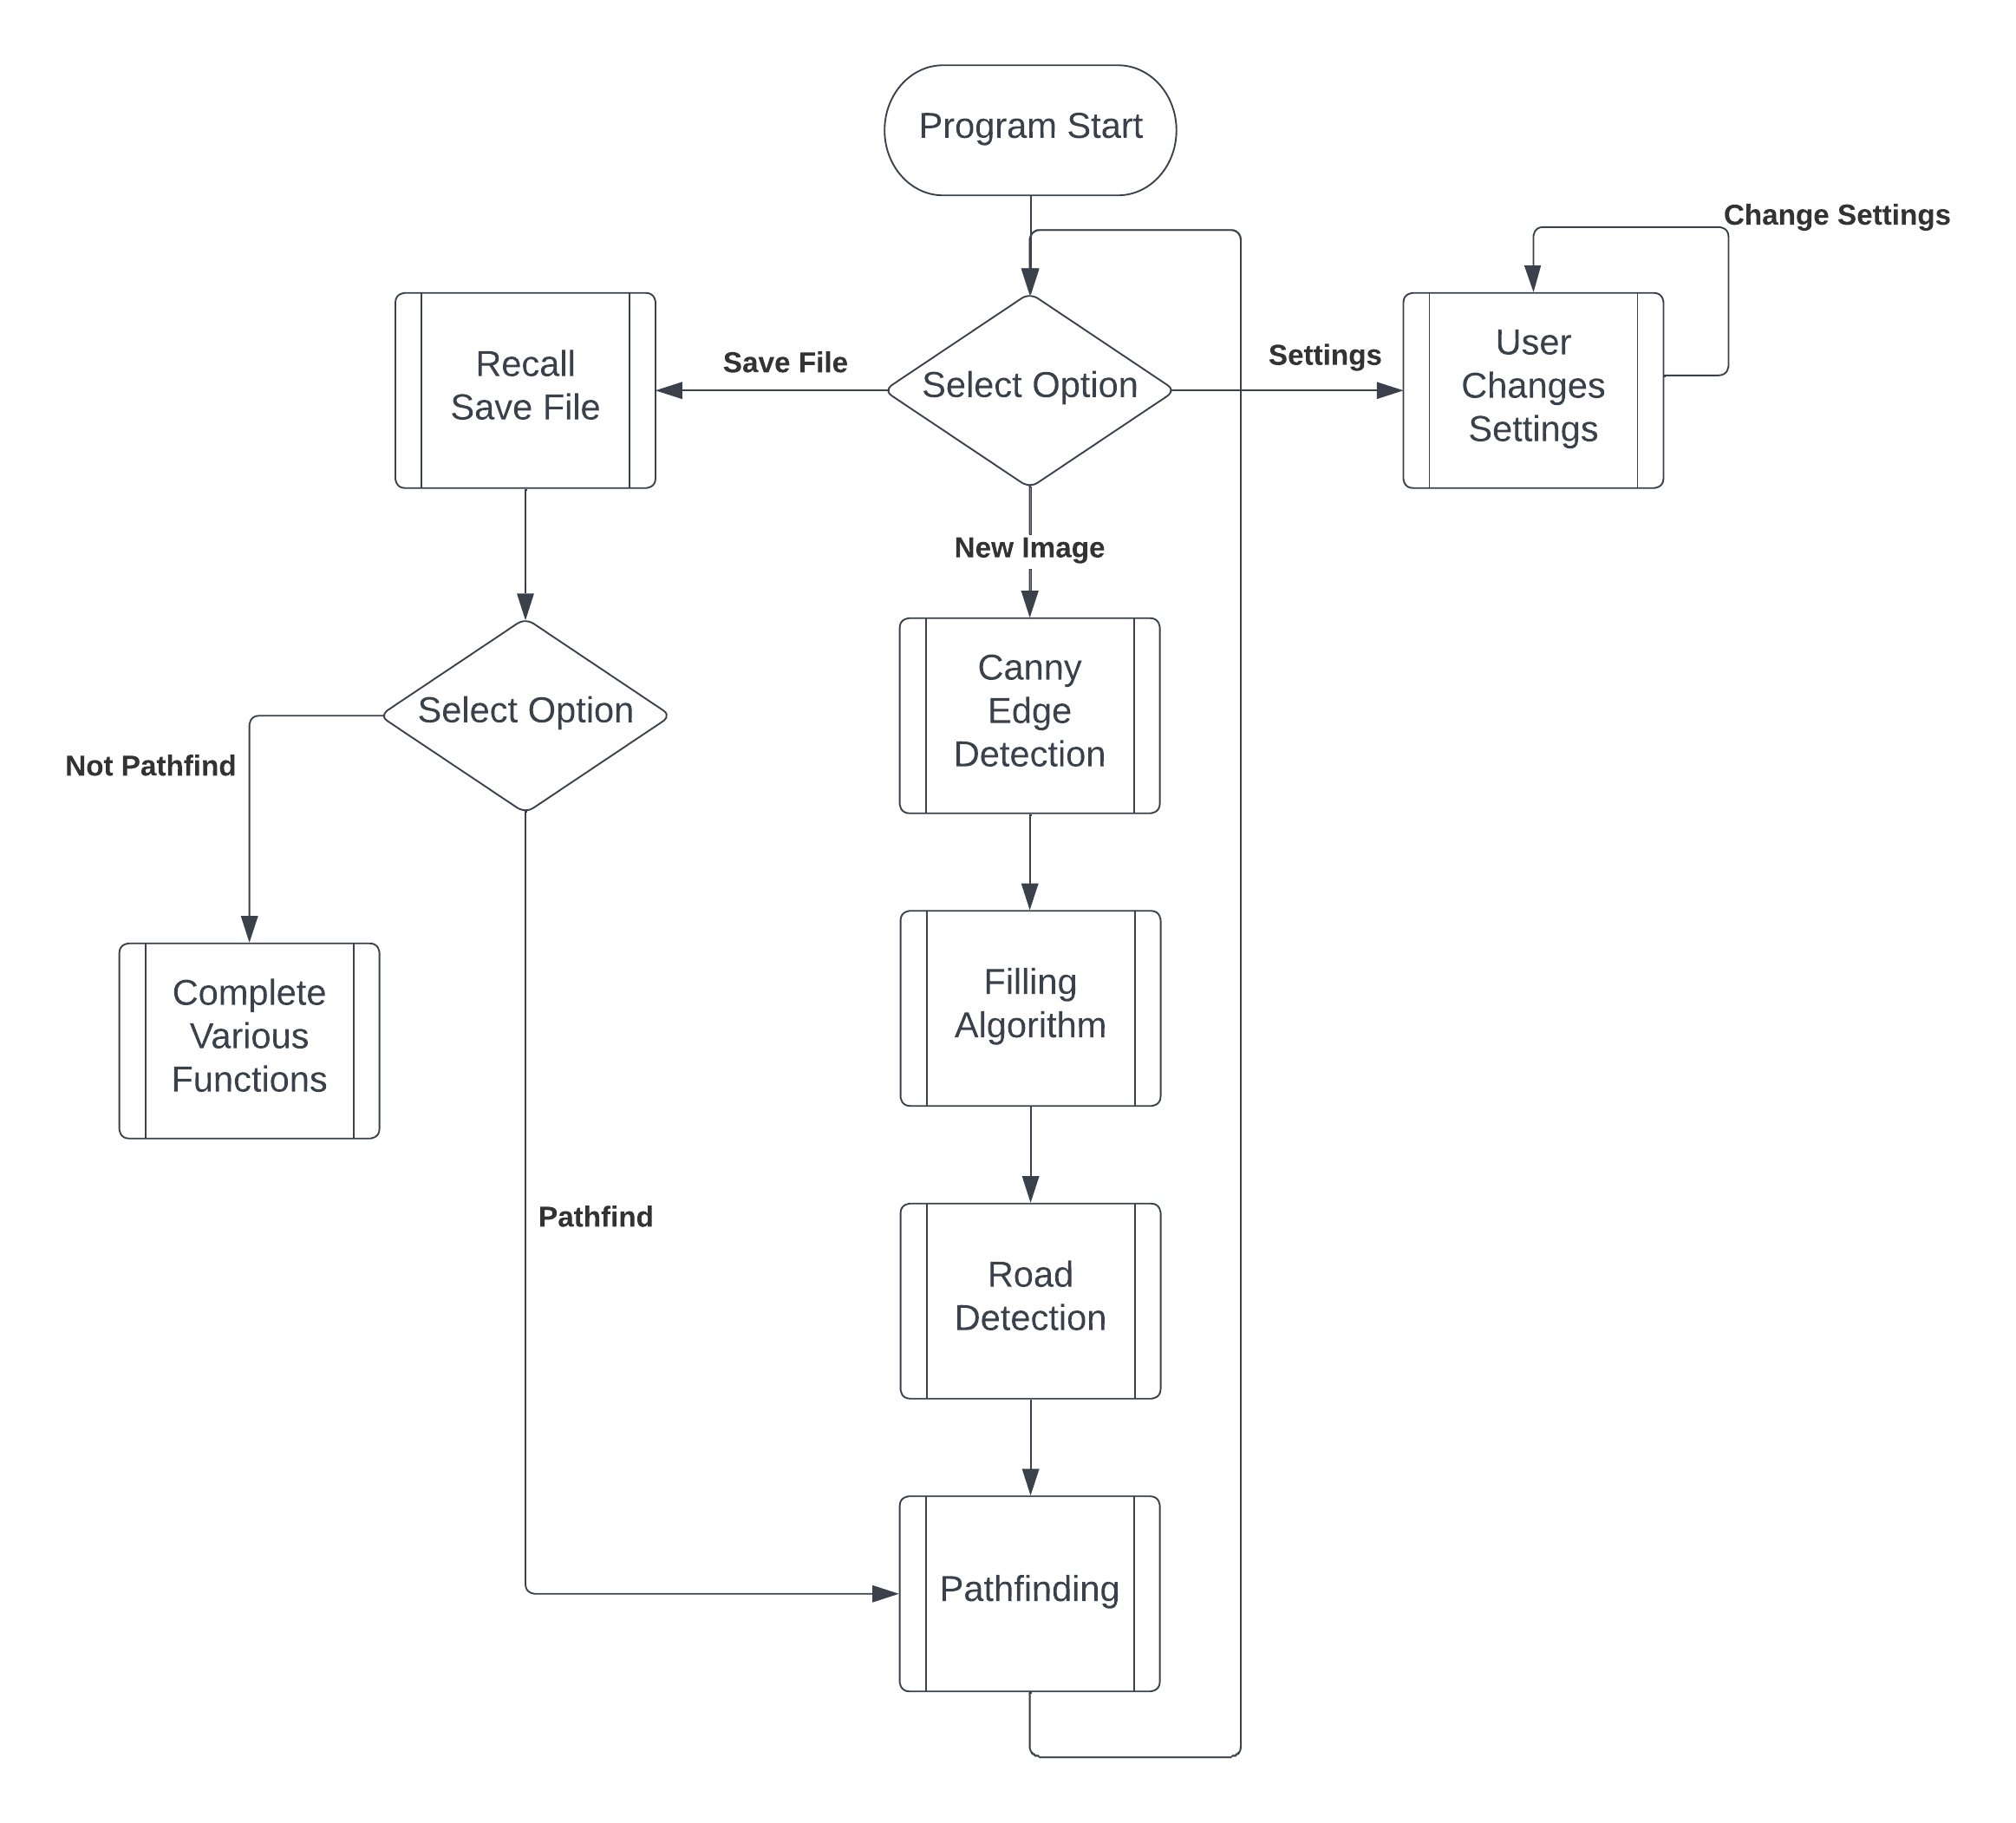
\includegraphics[width=17.2cm]{images/HighLevelOverview.png}}}
    \end{figure}

    The version of Edge Detection I will be using as previously stated will be Canny Edge Detection, this is as opposed to Sobel Edge Detection. The main version of filling I will be using is flood fill due to it simple nature to implement ad due to the fact that it does not take much memory and can be made recursive so it performs well. The final main algorithm I will need to use is image kernels and convolution, this will allow me to manipulate the inputted image.

    \subsubsection{Backend Library}
    For my project to ensure that I conform to the OOP principle of encapsulate what varies. I will accomplish this through the use of classes and encapsulation. Furthermore I have also made the decision to split up my solution into two separate projects, this means that my program will produce two files in order to run, one of these will be the DLL for the backend library and the other will be the executable for the front end. \\ \bk

    Contained within this backend section of my program will be contained the edge detection, road detection, complex data types and graph traversal algorithms as well as various utilities that are frequently used throughout the program. \\ \bk

    One of the main features of the backend library are the custom structures that have been created in order to allow for easier processing of data. Find below the image of the structure class layout and the classes which link within.

    \begin{figure}[H]
        \centering
        \subfloat[\centering Overview of Backend Structures]{{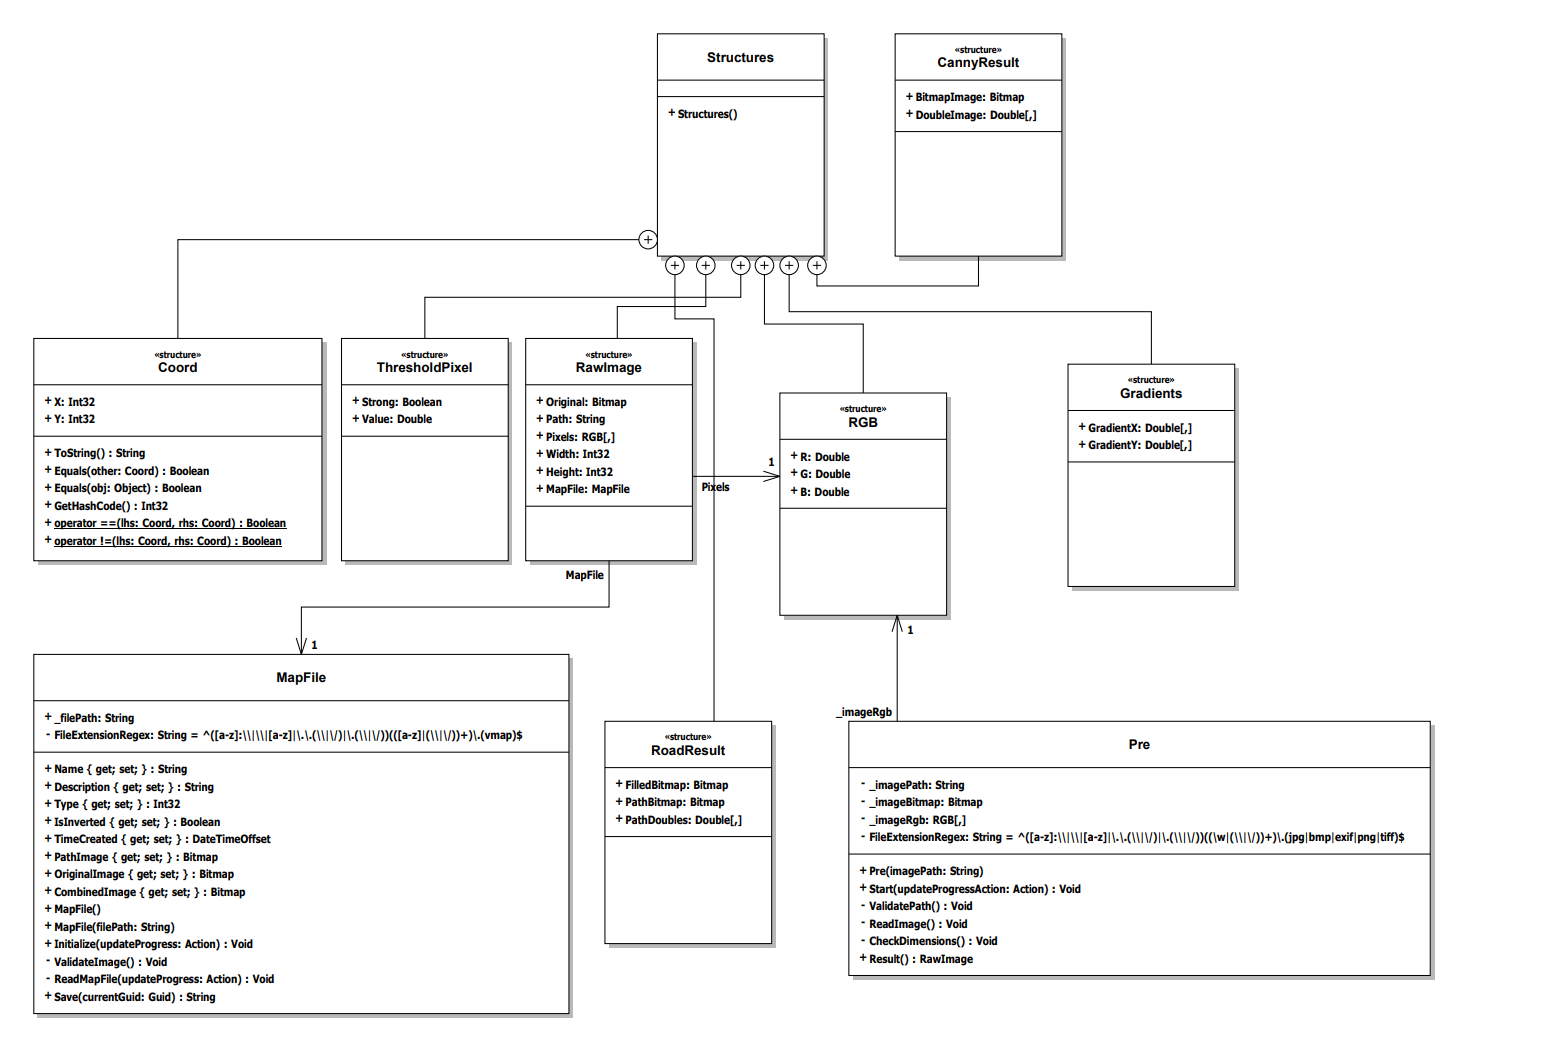
\includegraphics[width=17.2cm]{images/UML/Backend.png}}}
    \end{figure}

    \\

    As can be seen form the class diagram of the backend library, there is very little dependency within the library itself. This allows the backend to function independently of the program which is using it. This allows the backend to be split out and moved to another program if needed. Summarised there are four main reasons to do this:

    \begin{itemize}
        \item \textbf{Modularity} - By separating the backend from the frontend one is able to be built without the other. This means that when working on my project I can take time to perfect one without impacting the other.
        \item \textbf{Reusability} - As previously stated being able to be reused is a large reason as to why to separating the elements is a good idea. Since if I wanted to expand this project for example and make a web interface for it, I could take the maths of the backend and recreate the front end in a web framework like Razor Pages.
        \item \textbf{Maintainability} - It is allot easier to maintain code when it has been organised into classes and by extension into libraries where a library is a collection of classes. It means that should something throw an error in the backend I would be able to easily isolate the issue and be able to fix it.
        \item \textbf{Testability} - In a similar vain to the Maintainability of the program being modular also means that it is very easy to implement testing. This means that as I go thorough making my program it will make it allot easier to separate variables and make isolated testing conditions. Furthermore it means that I can test the maths of the Canny Detection without having to worry about making an interface to it using the UI.
    \end{itemize}
    \\ \BK

    \subsubsection{Local Application}
    The local application part of this program will be responsible for the tying if the various algorithms of the backend together along with providing the user with a way to interact with them, whether this is through the use of windows forms of the console for text inputs. As stated by objective 5 the design of the UI should be simplistic and easy to understand at a glance, therefore I will only be using the methods as stated above for interacting with the user. I also believe that it will be best to keep the changes between the two to a minimum and when there is a change make sure that the user is aware of it before hand.\\ \bk
    
    \paragraph{Design of User Interface (Console)} \mbox{} \\
    In order to keep the user interface as easy to use as possible the console will remain static while the program is being run. This means that once it has been started and set to its correct size it will form itself to fit the screen and will only run if it has been maximized. This will allow me to make sure that the interface is clear and easy to use. Find below a mock-up of the console design.
    
    \begin{figure}[H]
        \centering
        \subfloat[\centering Mock-up of Console Interface]{{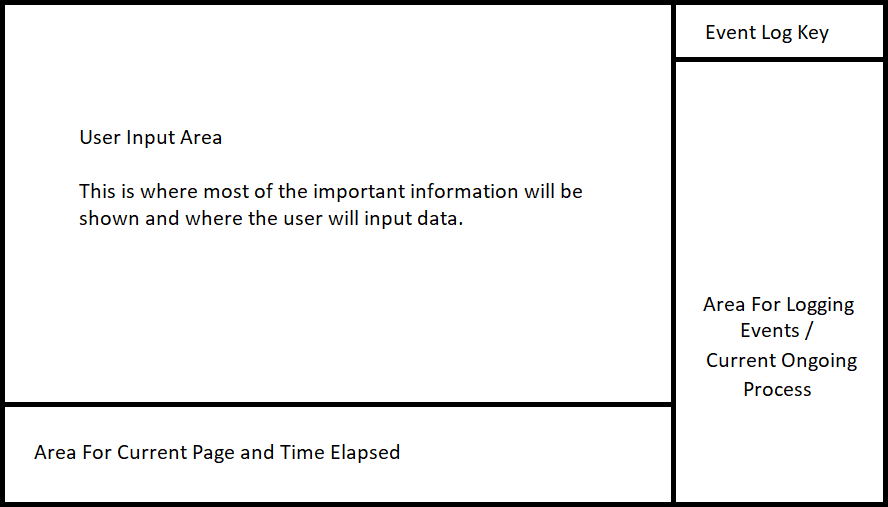
\includegraphics[width=12.5cm]{images/design/consoleMock.png}}}
    \end{figure}\\

    As can be seen in this mock-up fo the console interface it can be seen that there is a large section for the user to enter and view important in. As will be expanded on in the second section about the Windows Forms interface, due to the static nature of the console I will be able to make a Form conform to the shape of this area. See the next paragraph for more information. \\ \bk

    As for the other elements of the console UI, as part of objective 5, this must be easy to see at a glance what is going on and which step you are in. To accomplish this on the right hand side of the console there will be a log which, should the user select to do so in settings, will display each method call and the result of that call allowing them to see exactly where they are in the process. \\ \bk
    
    At the bottom of the console in the section labelled "Area for Current Page and Time Elapsed" this will be used for, as the name suggests, the current page and time elapsed. What this means is that at a glance a non-technical user or one who has opted not to have the advanced logging will still be able to see where they area at in the current process. \\ \bk

    \begin{figure}[H]
        \centering
        \subfloat[\centering Mock-up of Console Interface]{{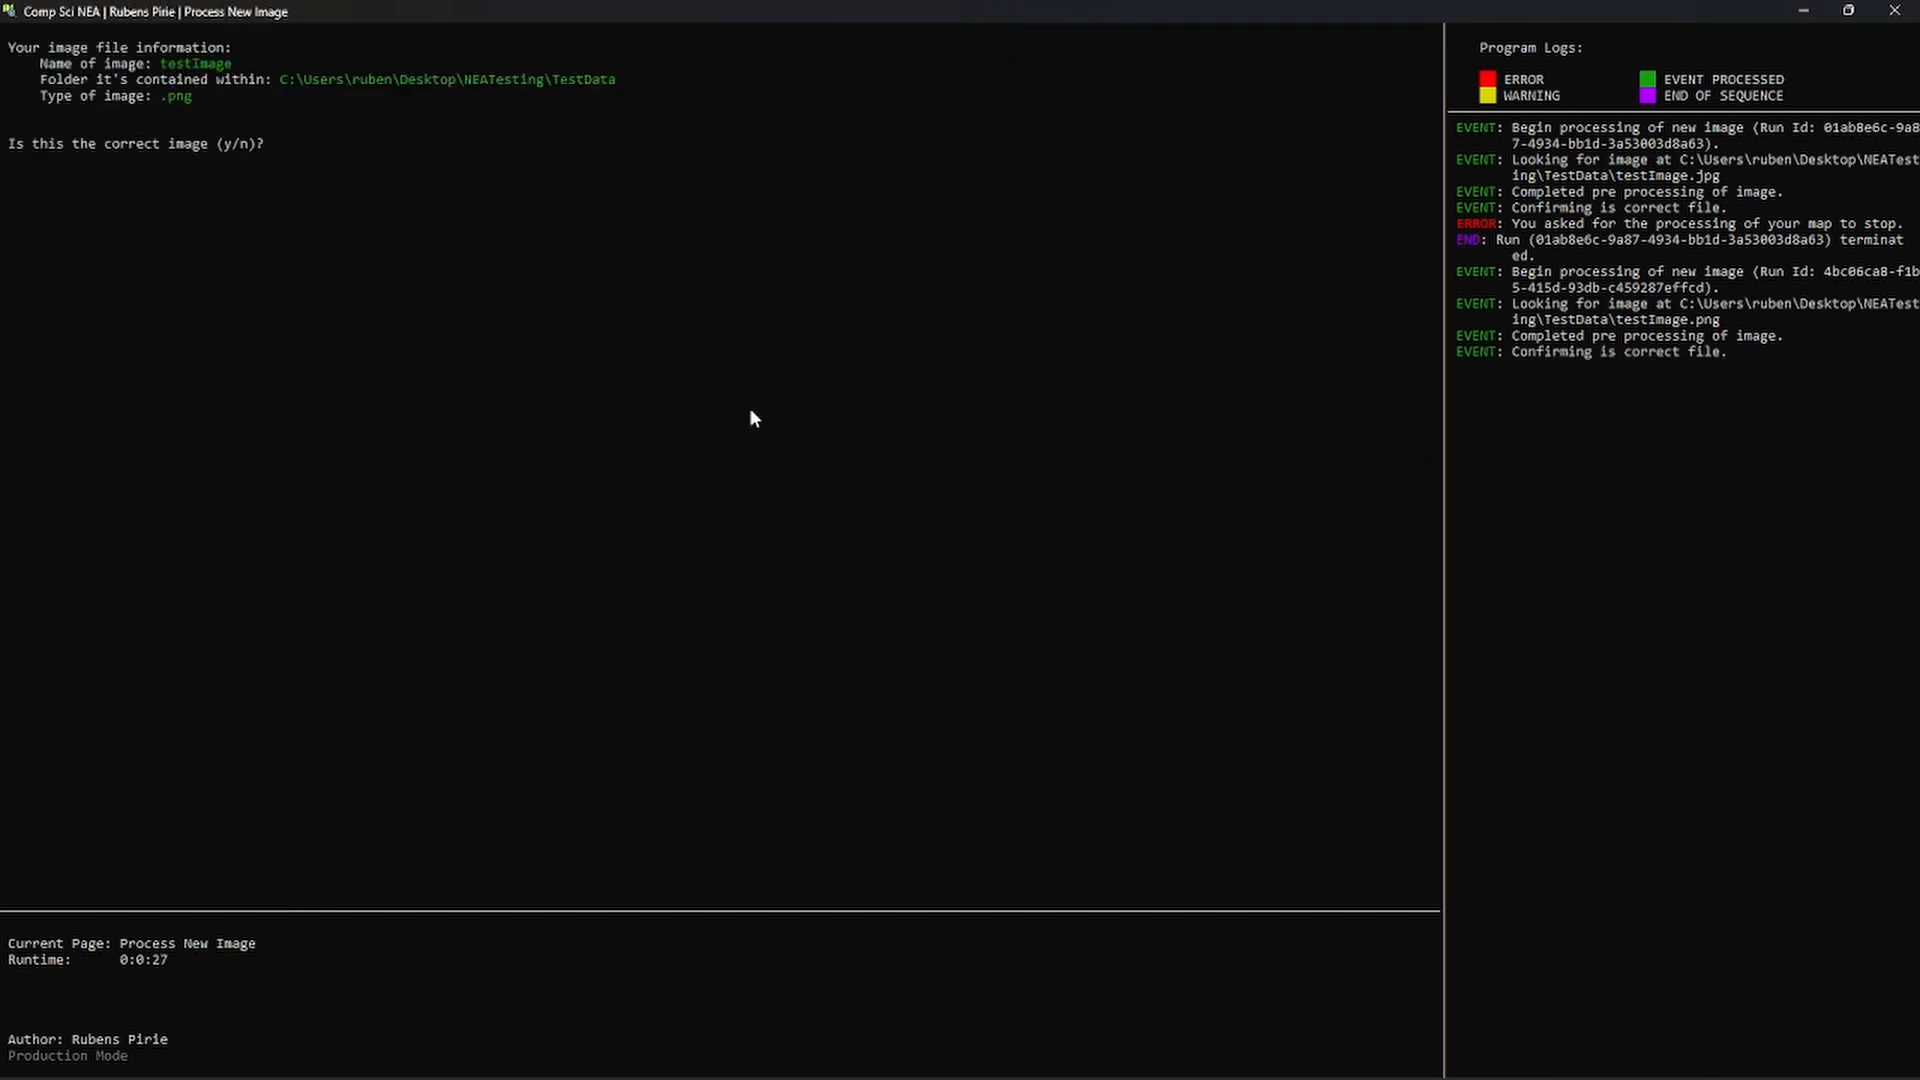
\includegraphics[width=12.5cm]{images/design/terminal.png}}}
    \end{figure}\\
    
    \BK

    \paragraph{Design of User Interface (Windows Forms)} \mbox{} \\
    For the forms interface I have chosen to keep the use of the opening of new windows to a minimum, as explained above I want this part of the program to be as simple as possible to avoid over stimulating the user and confusing them. 

    \begin{figure}[H]
        \centering
        \subfloat[\centering Windows Form For Confirming Image]{{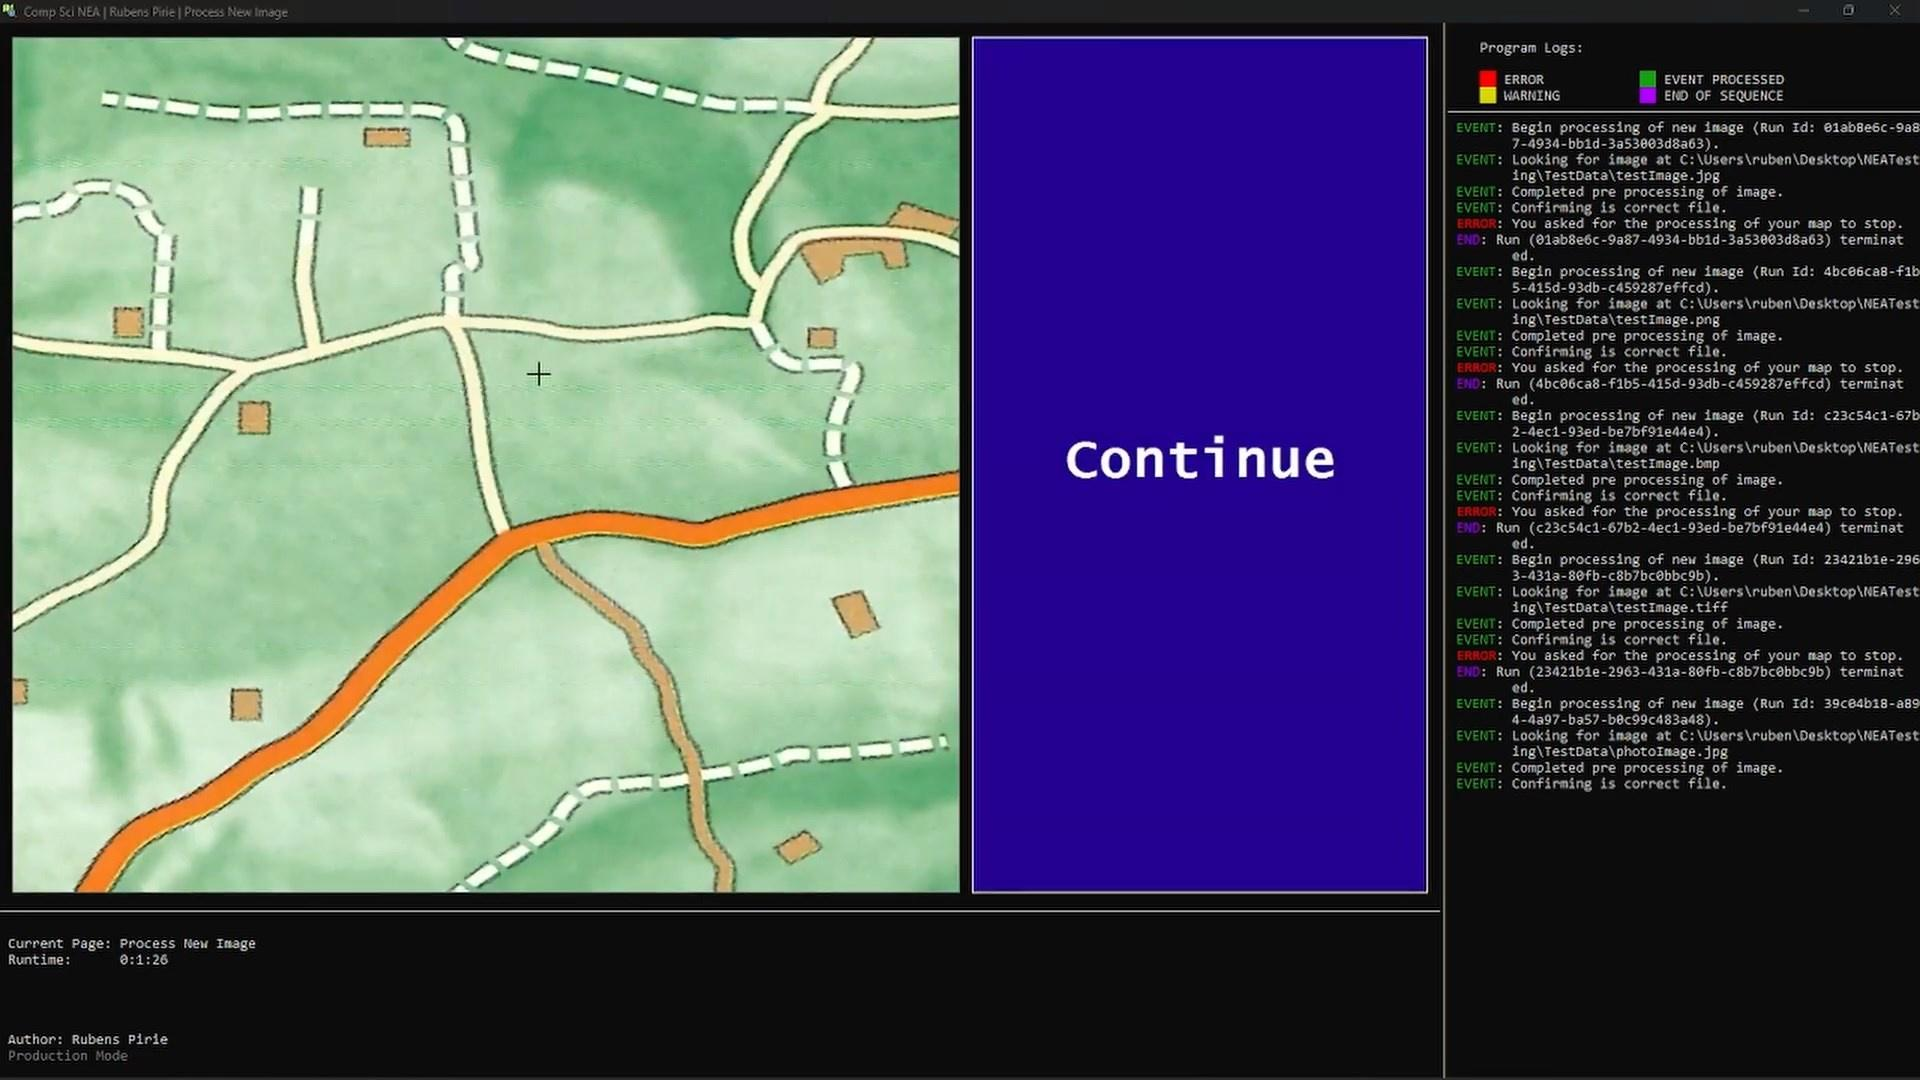
\includegraphics[width=12.5cm]{images/design/confirmWindow.jpeg}}}
    \end{figure}\\

    \begin{figure}[H]
        \centering
        \subfloat[\centering Windows Form For Pathfinding Image]{{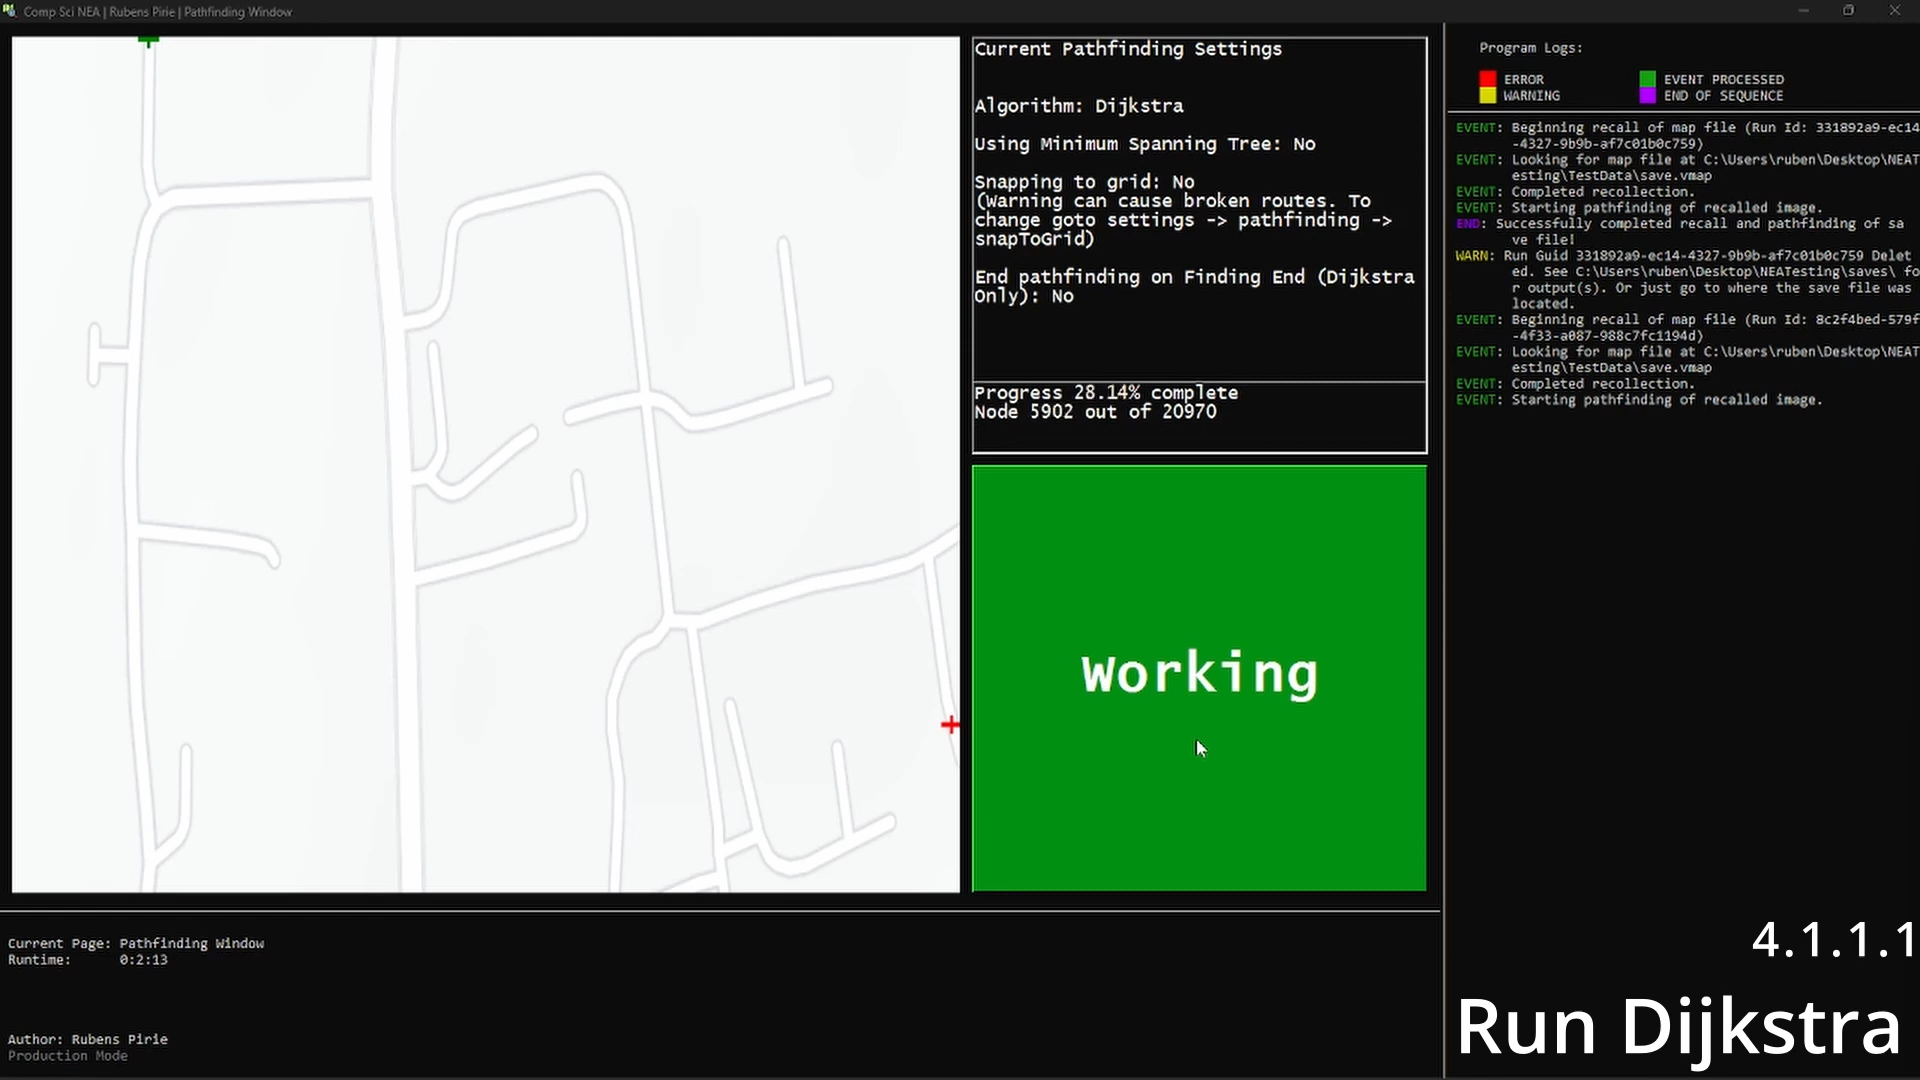
\includegraphics[width=12.5cm]{images/design/pathfindWindow.png}}}
    \end{figure}\\

    \\ \BK

    \subsubsection{Entire Class Diagram}
    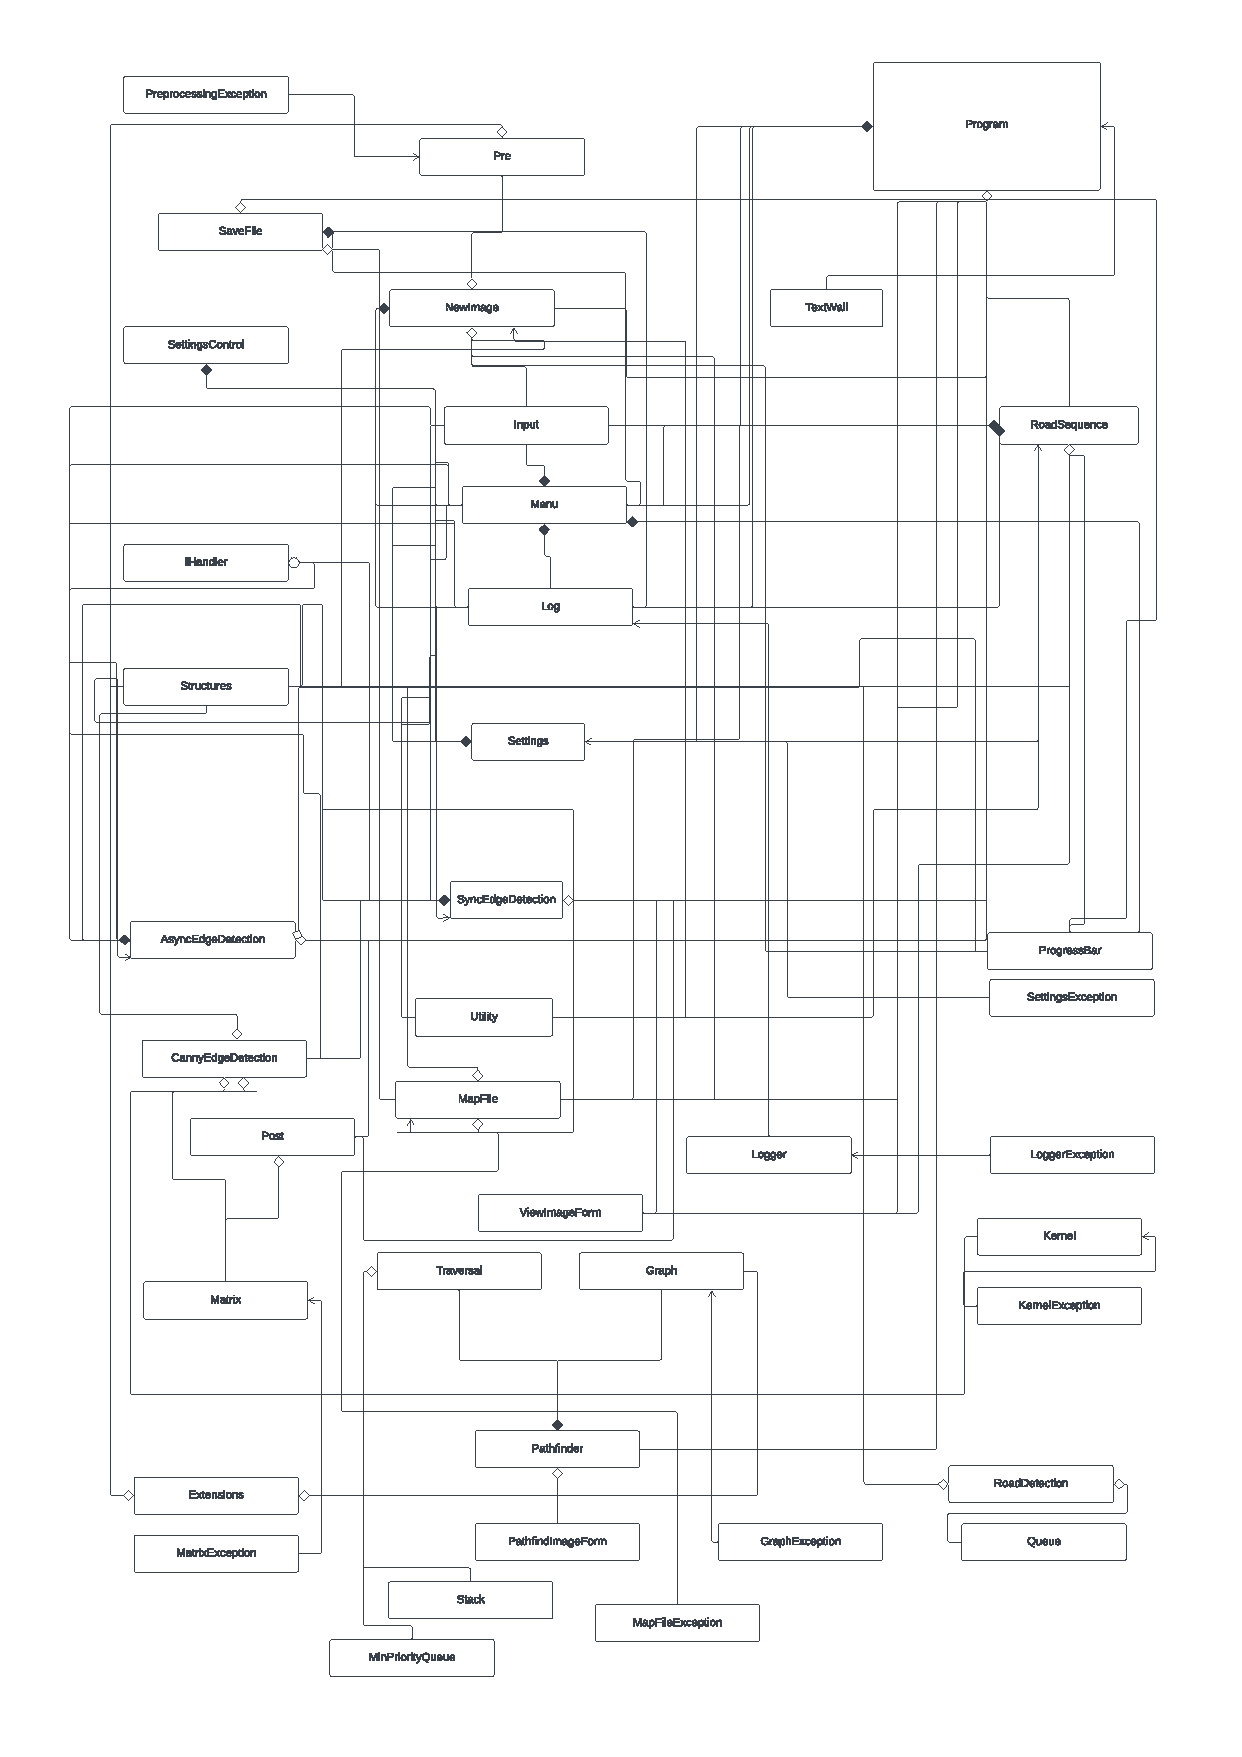
\includepdf{FullUML.pdf}
        
    \\ \bk

    \subsection{Class Overviews}

    In this following part of the write up will go briefly over every class in the program first stating its function, which section it is in (backend library or front end application) and finally how it plays a part in the program.

    \paragraph*{Async Edge Detection \textit{(Class)}} \mbox{} \\

    \begin{figure}[H]
        \centering
        \subfloat[\centering Async Edge Detection Class Diagram]{{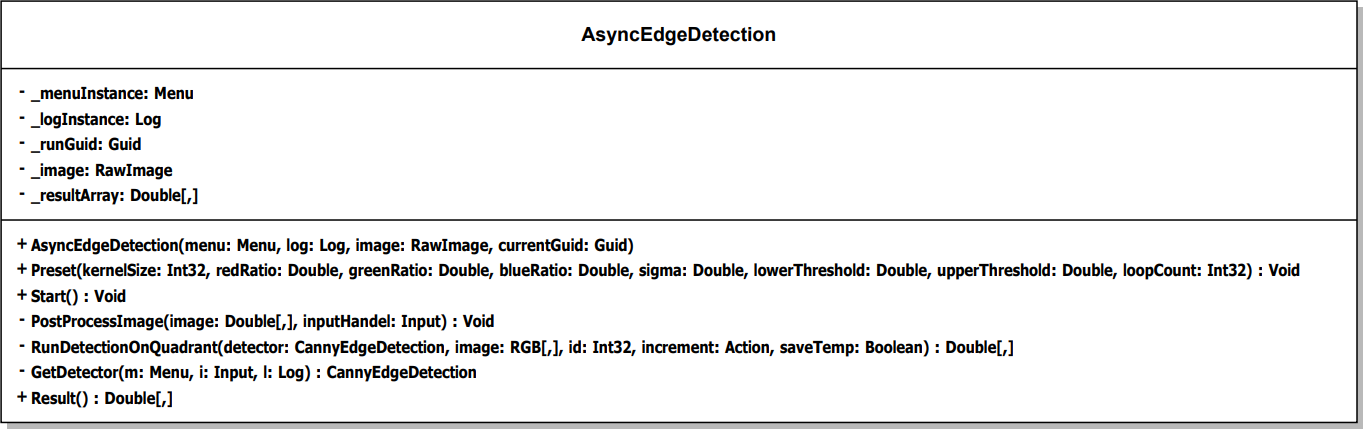
\includegraphics[width=16cm]{images/UML/AsyncEdgeDetection.png}}}
    \end{figure}\\

    This class is located in the front end section of my application, its main function is to coordinate the method calls of the Canny Edge Detection class. Due to the separated nature of my program I did not want there to be any user inputs in the accrual processing section. In order to do this I needed to have a separate hander on the local application side which would ask the user for their inputs and handel all of the validation of them. \\ \bk

    This class also implements the IHandler interface, this is to allow the main front end application to switch between the Async version and the Synchronous version of the edge detection without having a mess of IF statements. Part of the IHandler interface means that this class must contain the methods, Start() and Result(). What these methods do is what they say in the name. The start methods begins the process of getting user inputs and then starting the edge detection. The Result method will, as the name suggests return the result of the edge detection. \\ \bk

    The PostProcessImage method in the class is responsible for the custom embossing which runs through the result of the canny edge detection and fills in any gaps that may have appeared. It also applies an embossing kernel on the image to embolden the lines. It will also prompt the user to enter the amount of times they want to run the embossing process. \\ \bk
    
    The GetDetectorMethod is used to get the variables for the canny edge detector. This section handles all of the validation and checking that the values supplied are valid. The result of this method is that a new Canny Edge Detector object is created with the user inputted variables, this is then passed down the chain to be used in processing each quadrant. \\ \bk

    The main differentiator between this asynchronously method and the synchronous method is that this one will split the input image into 4 distinct quadrants, this will allow the program to run each at the same time using threading. Through my prototyping stage I found that using this method of threading greatly improves the speed even on lower specification computers. \\ \bk
    
    Finally the Preset method is used in the front end application in the eventuality of the user selecting preset values. An example of this is that when it gets to the selection of the edge detection method they select the "Photograph" method, the async method will be used due to its speed however instead of prompting the user it will run the various stages with predefined values. \\

    \bk


    \paragraph*{Canny Edge Detection \textit{(Class)}} \mbox{} \\

    \begin{figure}[H]
        \centering
        \subfloat[\centering Canny Edge Detection Class Diagram]{{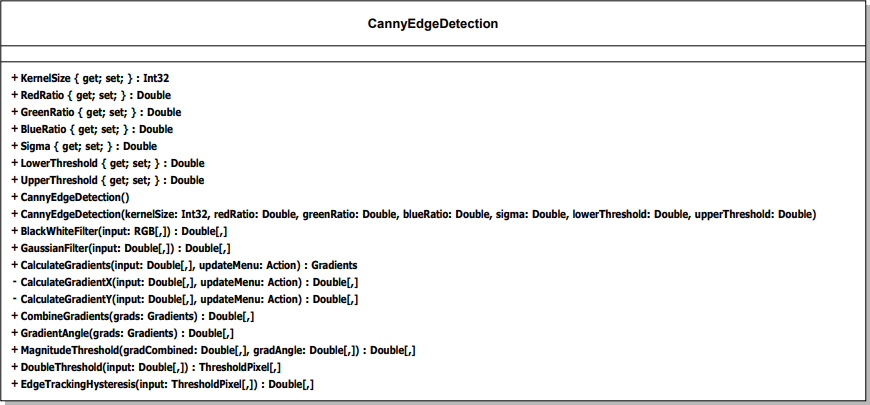
\includegraphics[width=16cm]{images/UML/CannyEdgeDetection.png}}}
    \end{figure}\\

    This class is located in the backend library portion of my project, its main function is to house the methods which contain the maths to perform the canny edge detection. Since this method is in the backend library of my project there is no user input here however in many of the methods an action is passed in, this is used to update the progress bar on the front end without having the two intrinsically integrated. \\ \bk

    The first set of methods shown in the class diagram are in essence properties on the class which are used in the various calculations. The reason that I will go with getter and setter variables is that if at some point in the future I wish to restrict access to the properties on the class or perhaps mutate the way in which they are stored this could be easily done without the need to change many different things. \\ \bk

    The first method and subsequently the first stage in canny edge detection is the black and white filter. The default behaviour is that it uses the industry standard for getting a single value from a RGB pixel which is as follows $$ Y' = 0.299R' + 0.587G' + 0.114B' $$.  It will perform the same calculation for every pixel in the supplied image causing it to be converted to black and white. This is used since if the detection was run on each colour chanel seperatly this would not give one unified result and could be very inaccurate.\\ 

    \\ \bk

    The next method in this class is the Gaussian Filter this will pass over the image and apply a Gaussian Filter kernel to each pixel. This is mainly used in order to make sure that any noise in the image is suppressed to avoid false edges. The maths for the kernel implementation and matrix convolutions are covered in their respective classes as well as the gaussian equation. A rough approximation for the gaussian kernel is as follows:\\

    \begin{gather*}
        \frac{1}{159}\begin{pmatrix}
            2 & 4 & 5 & 4 & 2 \\
            4 & 9 & 12 & 9 & 4 \\
            5 & 12 & 15 & 12 & 5 \\
            4 & 9 & 12 & 9 & 4 \\
            2 & 4 & 5 & 4 & 2
        \end{pmatrix}
    \end{gather*} \\

    It is stated that the larger the kernel is the less effect noise will have on the result however it will impact the performance of the detector, for this reason the Canny Edge Detection class defaults to a kernel size of 5x5. \\ \bk

    The next stage of canny edge detection involve calculating gradients and gradient angles and for this reason I will be combining the CalculateGradients, CalculateGradientX and CalculateGradientY into one. Again another way in which I will optimise the canny edge detection is by using threading. In order to calculate the gradient direction I will need to use Atan2, this requires an X and Y component which are independent of each other, a perfect use of threading. When a image gets to this point it will be processed at the same time by each method. The process completed by each method is vastly the same they will just be applying different image kernels, both are the sobel edge kernels keeping with the scheme of canny edge detection. \\ \bk   

    \begin{center}
        
        $
        M_x = \begin{pmatrix}
            +1 & +2 & +1 \\
            0 & 0 & 0 \\
            -1 & -2 & -1
        \end{pmatrix}
    $ 
    and $ M_y = \begin{pmatrix}
            +1 & 0 & -1 \\
            +2 & 0 & -2 \\
            +1 & 0 & -1 
        \end{pmatrix}
    $
    \end{center} \\
 
    \bk

    Once the gradient magnitudes in each dimension have been calculated the result of these can be fed into the CombineGradients method. This method will finally extract the usefully data which has been created from applying the two sobel gradient kernels. The first of these is working out the combined gradient magnitudes which is simply calculated with the equation: \\
    
    \begin{gather*}
        G = \sqrt{G_x^2 + G_y^2}
    \end{gather*} \\
    
    We then also want to calculate the direction in which the gradient is travelling to work out if it is extreme enough to quantify an edge. This is achieved though the use of Atan2 as follows:\\
    
    \begin{gather*}
        \Theta = \text{Atan2}(G_x, G_y)
    \end{gather*} \\ 

    \bk

    The next stage in canny edge detection is gradient magnitude threshold's, this is a method of removing lines which would not be "thick enough" to be a propped edge. This is accomplished by the use of the MagnitudeThreshold method and the bullet point description: \\ 
    
    At every pixel N in a given image, it will be suppressed (removed) if,
    \begin{itemize}
        \item the rounded gradient angle is 0° (i.e. the edge is in the north-south direction) the point will be considered to be on the edge if its gradient magnitude is greater than the magnitudes at pixels in the east and west directions.
        \item the rounded gradient angle is 90° (i.e. the edge is in the east-west direction) the point will be considered to be on the edge if its gradient magnitude is greater than the magnitudes at pixels in the north and south directions.
        \item the rounded gradient angle is 135° (i.e. the edge is in the northeast-southwest direction) the point will be considered to be on the edge if its gradient magnitude is greater than the magnitudes at pixels in the north-west and south-east directions.
        \item the rounded gradient angle is 45° (i.e. the edge is in the northwest-southeast direction) the point will be considered to be on the edge if its gradient magnitude is greater than the magnitudes at pixels in the north-east and south-west directions.

    \end{itemize}
    
    \\ \bk

    The penultimate method call is to Double Threshold suppression. After the magnitude threshold, remaining edge pixels provide a more accurate representation of real edges in an image. However, some edge pixels remain that are caused by noise and color variation which didn't get removed by the gaussian filter stage. To account for these spurious responses, it is essential to filter out edge pixels with a weak gradient value and preserve edge pixels with a high gradient value. \\

    The way in which this is implemented is that a user threshold from the beginning is used and if the pixel is greater than the threshold then it is included, if it is below the max threshold but greater than the min then it is set to a strong pixel and retains its value. In any other case it is removed and its value is set to 0. \\ \bk

    Finally edge tracking by hysteresis is used, to track the edge connection, blob analysis is applied by looking at a weak edge pixel and its 8-connected neighbourhood pixels. As long as there is one strong edge pixel that is involved in the blob, that weak edge point can be identified as one that should be preserved. These weak edge pixels become strong edges that can then cause their neighbouring weak edge pixels to be preserved otherwise they are not preserved and are removed. After each of these sages canny edge detection is complete. \\ \bk    
    \bk


    \paragraph*{Canny Result \textit{(Structure)}} \mbox{} \\

    \begin{figure}[H]
        \centering
        \subfloat[\centering Canny Result Class Diagram]{{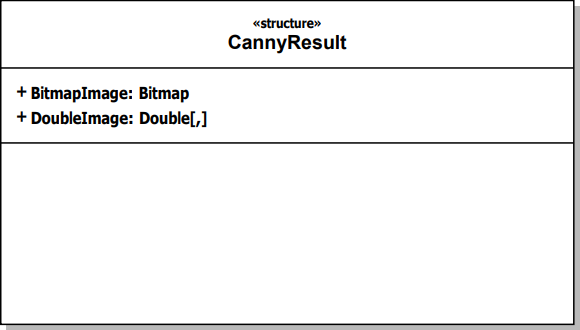
\includegraphics[width=8cm]{images/UML/CannyResult.png}}}
    \end{figure}\\

    This is contained within the static class of structures in the backend library. There is no methods or functions contained within this class since it is in fact a structure. Its main function is to contain any relevant data from Canny Edge Detection.

    \bk

    \paragraph*{Coord \textit{(Structure)}} \mbox{} \\

    \begin{figure}[H]
        \centering
        \subfloat[\centering Coord Class Diagram]{{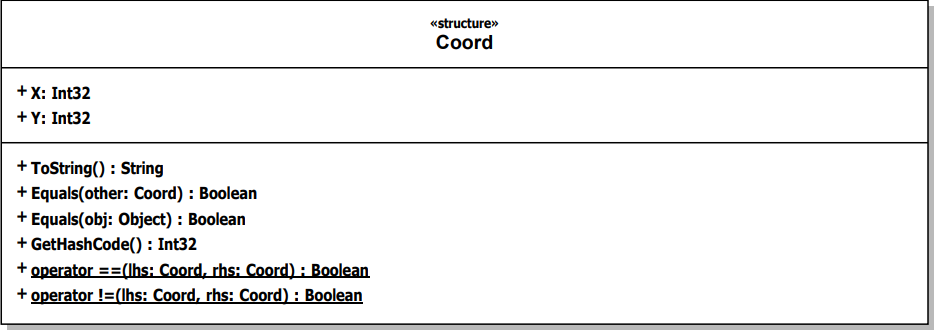
\includegraphics[width=13cm]{images/UML/Coord.png}}}
    \end{figure}\\

    Similar to above this is contained within the static class of structures. It is used to represent a coordinate, and unlike the canny result structure, it does contain methods. The main of which are the operator overloads. This allows me to directly compare two different coordinates instead of constantly comparing each dimensions. The other hash codes and alike are used when a dictionary is required in order for them to be converted into a hash code. Finally the ToString method is mainly used during testing however it can also be used to inform the user of a coordinate that they are interacting with.

    \bk

    \paragraph*{Extensions \textit{(Class)}} \mbox{} \\

    \begin{figure}[H]
        \centering
        \subfloat[\centering Extensions Class Diagram]{{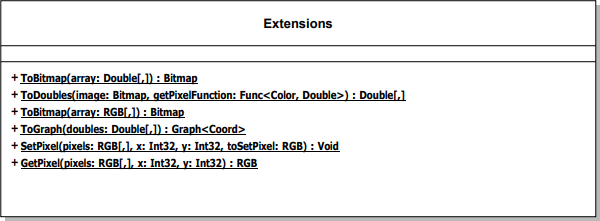
\includegraphics[width=13cm]{images/UML/Extensions.png}}}
    \end{figure}\\

    This class is responsible for altering the default behaviors of certain inbuilt classes in C# as well as extending functionality to make it easier to maintain my code. The way in which this is achieved is through the use of the this keyword. It will allow me for example to be to .ToBitmap on a 2D array speeding up the process instead of calling separate methods.\\ \bk

    The first of the extensions that will be implemented is the ToBitmap extension. As stated above it allows me to call ToBitmap on any given 2D double array, it then converts it to a bitmap and returns said bitmap. It does this through taking each pixel in turn and then using the Utility method to bound them within the allowed range of a pixel. \\ \bk

    Another of the extensions contained within this class is the ToDoubles extension which is essentially the inverse of the ToBitmap extension. This acts upon a Bitmap to convert it to a 2D double array. This extension however requires a method to be passed in which is then used to work out how to get the values of the pixel to a single 0 -> 255 value. The function which is passed in must take a Color object and return a single double value. \\ \bk

    The third extension contained is essentially a clone of the first one however this acts upon the EGB structure. This is important due to the fact that the RGB structure contains more than 1 value which means that using it I can reconstruct the original image using the R, G and B channels in the structure. Apart from this difference the two extensions are the same. \\ \bk

    The ToGraph extension contained within this class is very important as it is how after the canny edge detection I will convert the result to a graph which can then have a traversal algorithm used upon it. This extension acts upon a 2D double array. In order to gain the pixels around a given pixel in a double array the GetKernel function is used, this is explained in the Kernel class. Once the kernel of the pixel is created we can work out the relative coordinates through the use of modulus arithmetic.

    \begin{gather*}
        \text{Where } X = x + (i \% 3) -1 \text{ and } Y = y + (i / 3) - 1 \\
    \end{gather*} \\ 

    Once this has been calculated more maths is done however this is contained within the graph class so see there for more information. \\ \bk

    The next two structures go hand in hand so I will talk about both of them together, due to the image processing and the way in which I am accessing the arrays which contain the data I feel that it would be easier if I could alter my RGB[,] and directly access it with the .setPixel and .getPixel methods since this is how it is used in the bitmap class. Therefore it would make it easier to use the two interchangeably instead of accessing it using direct accessing then changing the value. The way in which they both work is that in the function call an x and y coordinate is passed as well as a colour if it is the set pixel version. Then it changes or returns the value.\\    

    \bk

    \paragraph*{Gradients \textit{(Structure)}} \mbox{} \\

    \begin{figure}[H]
        \centering
        \subfloat[\centering Gradients Class Diagram]{{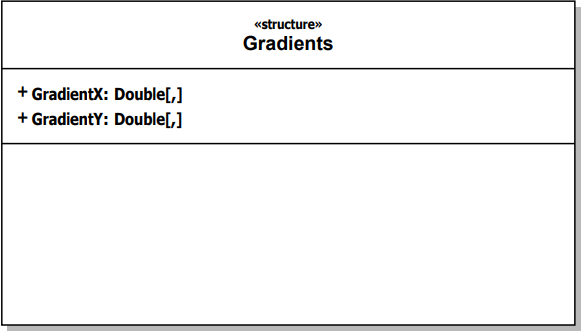
\includegraphics[width=8cm]{images/UML/Gradients.png}}}
    \end{figure}\\

    This is a structure located in the back end library of my project, its main function in the program is store the result of the gradient calculations. As with many of my structures in this code, there is no methods contained within. 

    \bk


    \paragraph*{Graph \textit{(Class)}} \mbox{} \\

    \begin{figure}[H]
        \centering
        \subfloat[\centering Graph Class Diagram]{{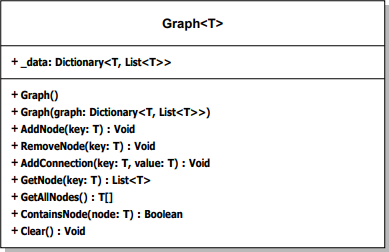
\includegraphics[width=8cm]{images/UML/Graph.png}}}
    \end{figure}\\

    \bk

    \paragraph*{Graph Exception \textit{(Exception)}} \mbox{} \\

    \begin{figure}[H]
        \centering
        \subfloat[\centering Graph Exception Class Diagram]{{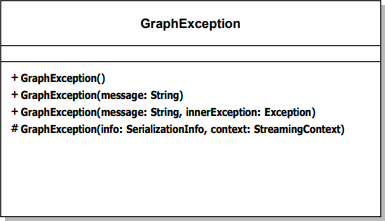
\includegraphics[width=12.5cm]{images/UML/GraphException.png}}}
    \end{figure}\\

    \bk

    \paragraph*{IHandler \textit{(Interface)}} \mbox{} \\

    \begin{figure}[H]
        \centering
        \subfloat[\centering IHandler UML Diagram]{{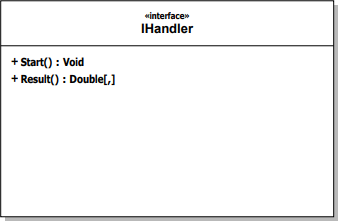
\includegraphics[width=12.5cm]{images/UML/IHandler.png  }}}
    \end{figure}\\

    \bk

    
    \paragraph*{Input \textit{(Class)}} \mbox{} \\

    \begin{figure}[H]
        \centering
        \subfloat[\centering Input Class Diagram]{{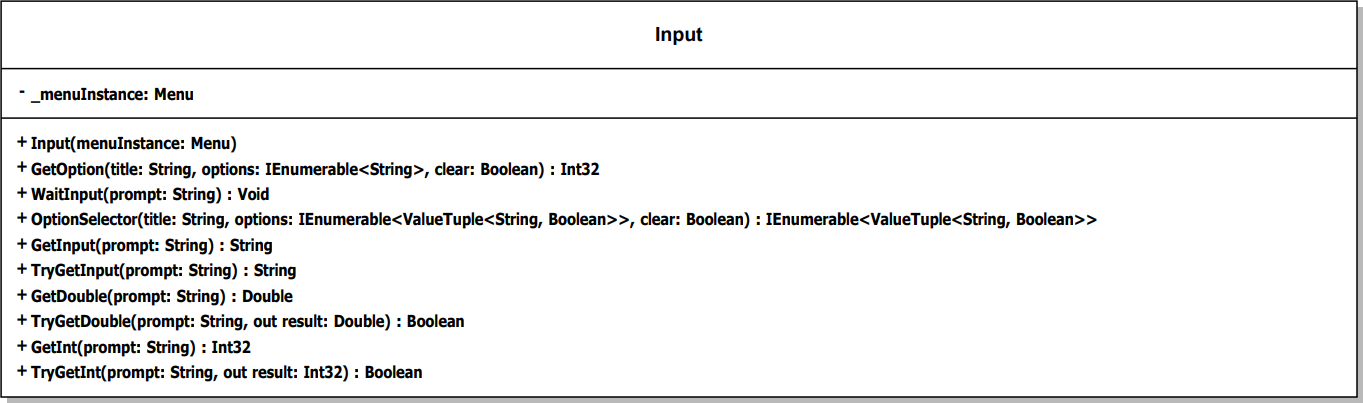
\includegraphics[width=12.5cm]{images/UML/Input.png}}}
    \end{figure}\\

    \bk

    
    \paragraph*{Kernel \textit{(Class)}} \mbox{} \\

    \begin{figure}[H]
        \centering
        \subfloat[\centering Kernel Class Diagram]{{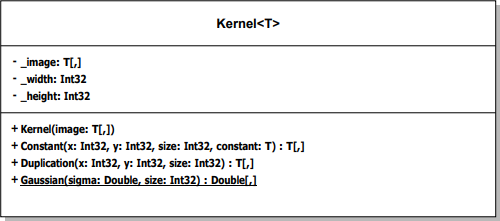
\includegraphics[width=12.5cm]{images/UML/Kernel.png}}}
    \end{figure}\\

    \bk

    
    \paragraph*{Kernel Exception \textit{(Exception)}} \mbox{} \\

    \begin{figure}[H]
        \centering
        \subfloat[\centering Kernel Exception Class Diagram]{{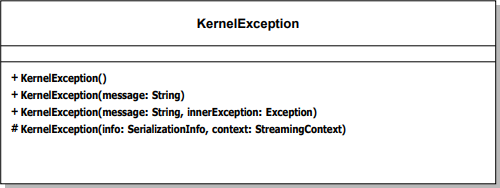
\includegraphics[width=12.5cm]{images/UML/KernelException.png}}}
    \end{figure}\\

    \bk

    \paragraph*{Log \textit{(Class)}} \mbox{} \\

    \begin{figure}[H]
        \centering
        \subfloat[\centering Log Class Diagram]{{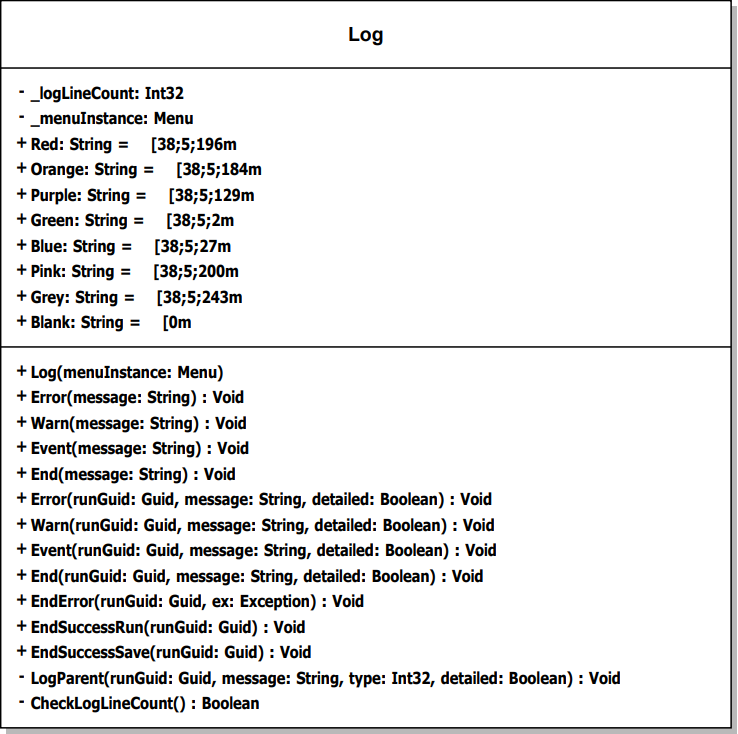
\includegraphics[width=12.5cm]{images/UML/Log.png}}}
    \end{figure}\\

    \bk

    \paragraph*{Logger \textit{(Class)}} \mbox{} \\

    \begin{figure}[H]
        \centering
        \subfloat[\centering Logger Class Diagram]{{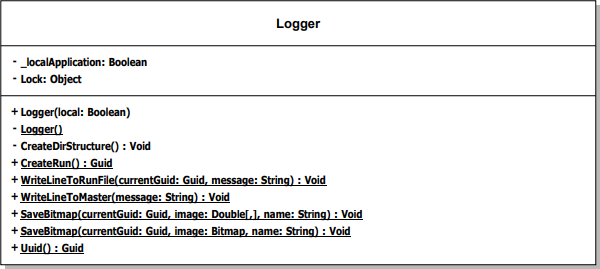
\includegraphics[width=12.5cm]{images/UML/Logger.png}}}
    \end{figure}\\

    \bk

    \paragraph*{Logger Exception \textit{(Exception)}} \mbox{} \\

    \begin{figure}[H]
        \centering
        \subfloat[\centering Logger Exception Class Diagram]{{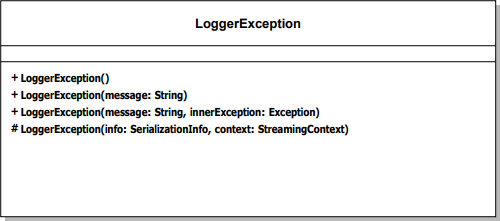
\includegraphics[width=12.5cm]{images/UML/LoggerException.png}}}
    \end{figure}\\

    \bk

    \paragraph*{Map File \textit{(Class)}} \mbox{} \\

    \begin{figure}[H]
        \centering
        \subfloat[\centering Map File Class Diagram]{{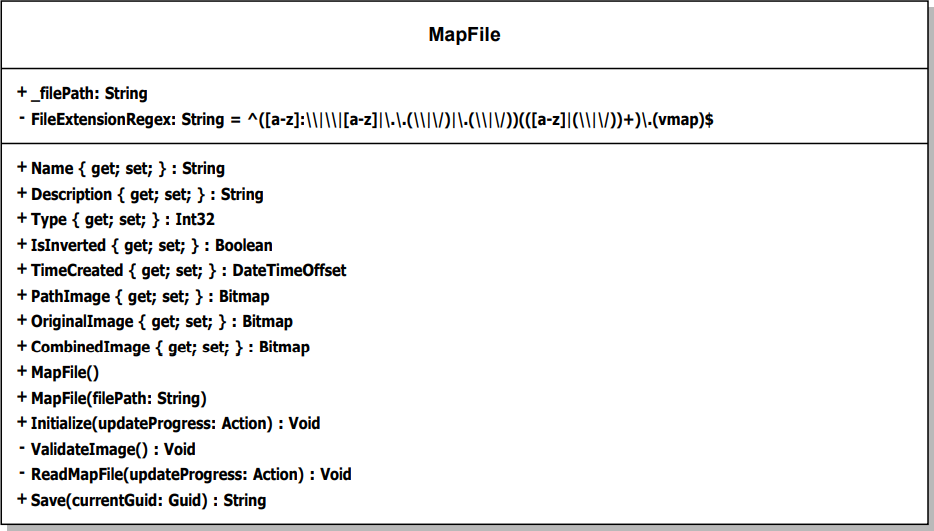
\includegraphics[width=12.5cm]{images/UML/MapFile.png}}}
    \end{figure}\\

    \bk


    \paragraph*{Map File Exception \textit{(Exception)}} \mbox{} \\

    \begin{figure}[H]
        \centering
        \subfloat[\centering Map File Exception Class Diagram]{{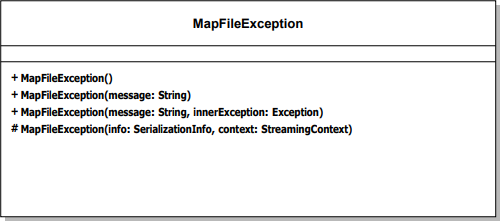
\includegraphics[width=12.5cm]{images/UML/MapFileException.png}}}
    \end{figure}\\

    \bk

    \paragraph*{Matrix \textit{(Class)}} \mbox{} \\

    \begin{figure}[H]
        \centering
        \subfloat[\centering Matrix Class Diagram]{{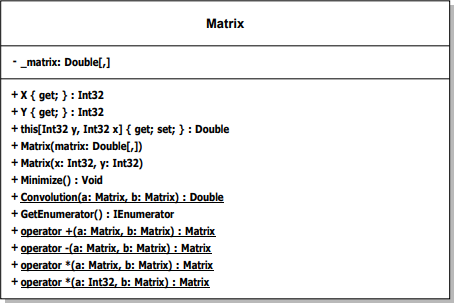
\includegraphics[width=12.5cm]{images/UML/Matrix.png}}}
    \end{figure}\\

    \bk

    \paragraph*{Matrix Exception \textit{(Exception)}} \mbox{} \\

    \begin{figure}[H]
        \centering
        \subfloat[\centering Matrix Exception Class Diagram]{{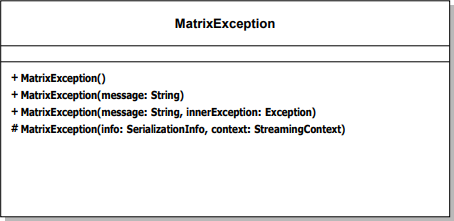
\includegraphics[width=12.5cm]{images/UML/MatrixException.png}}}
    \end{figure}\\

    \bk


    \paragraph*{Max Priority Queue \textit{(Class)}} \mbox{} \\

    \begin{figure}[H]
        \centering
        \subfloat[\centering Max Priority Queue Class Diagram]{{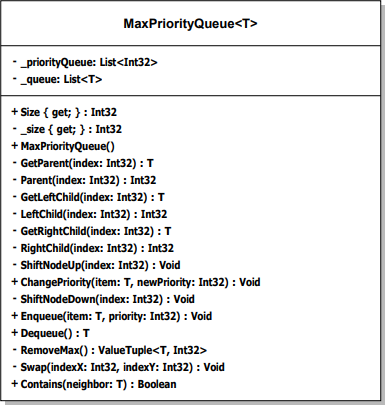
\includegraphics[width=12.5cm]{images/UML/MaxPriorityQueue.png}}}
    \end{figure}\\

    \bk

    \paragraph*{Menu \textit{(Class)}} \mbox{} \\

    \begin{figure}[H]
        \centering
        \subfloat[\centering Menu Class Diagram]{{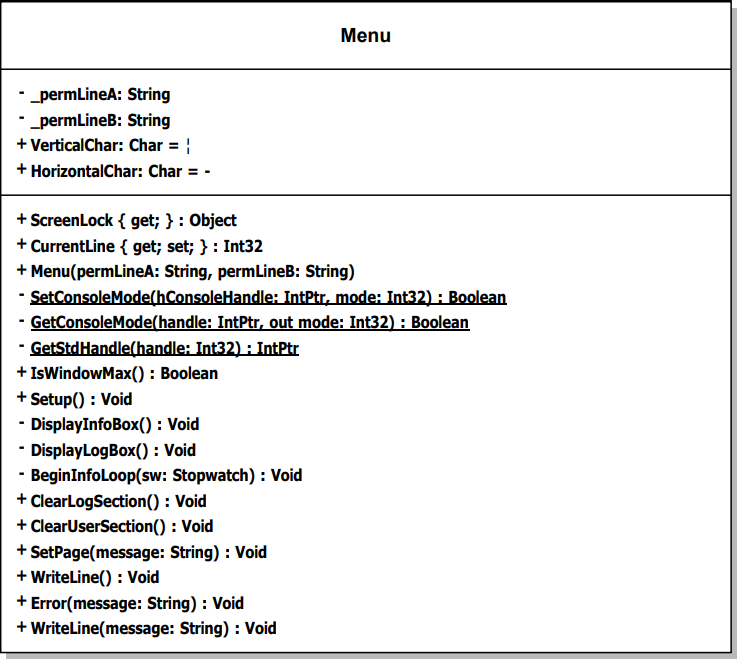
\includegraphics[width=12.5cm]{images/UML/Menu.png}}}
    \end{figure}\\

    \bk
    
    \paragraph*{Min Priority Queue \textit{(Class)}} \mbox{} \\

    \begin{figure}[H]
        \centering
        \subfloat[\centering Min Priority Queue Class Diagram]{{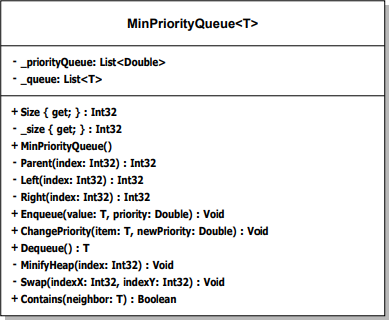
\includegraphics[width=12.5cm]{images/UML/MinPriorityQueue.png}}}
    \end{figure}\\

    \bk

    \paragraph*{New Image \textit{(Class)}} \mbox{} \\

    \begin{figure}[H]
        \centering
        \subfloat[\centering New Image Class Diagram]{{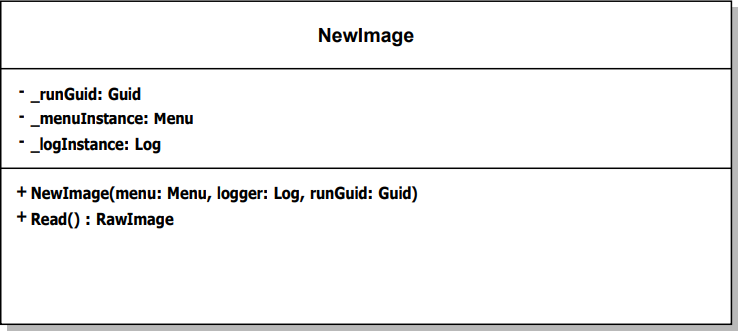
\includegraphics[width=12.5cm]{images/UML/NewImage.png}}}
    \end{figure}\\

    \bk

    \paragraph*{Pathfinder \textit{(Class)}} \mbox{} \\

    \begin{figure}[H]
        \centering
        \subfloat[\centering Pathfinder Class Diagram]{{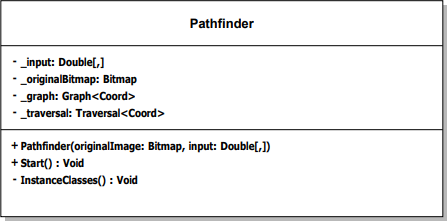
\includegraphics[width=12.5cm]{images/UML/Pathfinder.png}}}
    \end{figure}\\

    \bk

    \paragraph*{Pathfind Image Form \textit{(Windows Form)}} \mbox{} \\

    \begin{figure}[H]
        \centering
        \subfloat[\centering Pathfind Image Form UML Diagram]{{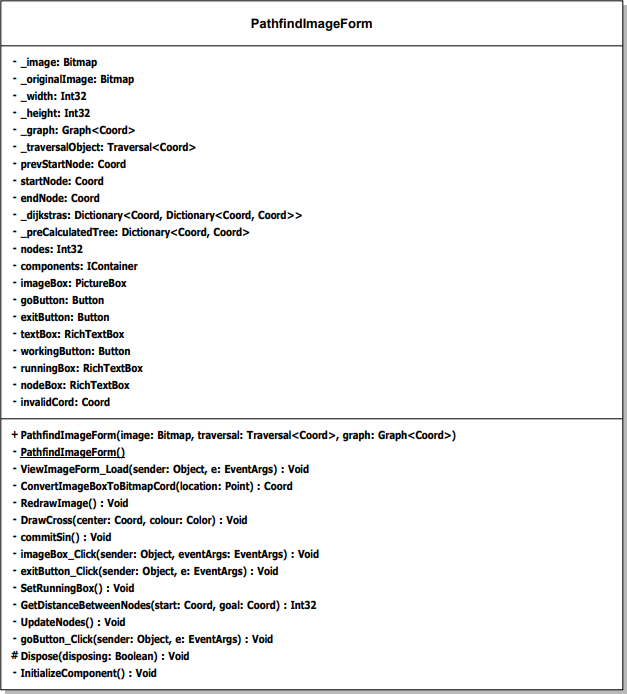
\includegraphics[width=12.5cm]{images/UML/PathfindImageForm.png}}}
    \end{figure}\\

    \bk

    \paragraph*{Post \textit{(Class)}} \mbox{} \\

    \begin{figure}[H]
        \centering
        \subfloat[\centering Post Class Diagram]{{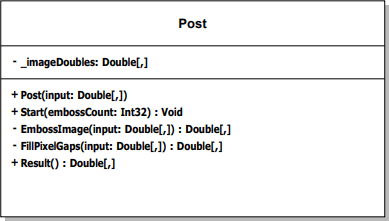
\includegraphics[width=12.5cm]{images/UML/Post.png}}}
    \end{figure}\\

    \bk

    \paragraph*{Pre \textit{(Class)}} \mbox{} \\

    \begin{figure}[H]
        \centering
        \subfloat[\centering Pre Class Diagram]{{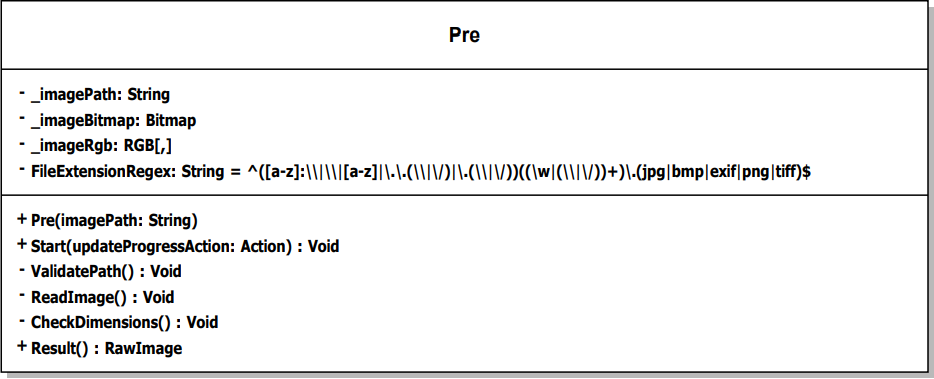
\includegraphics[width=12.5cm]{images/UML/Pre.png}}}
    \end{figure}\\

    \bk

    \paragraph*{Preprocessing Exception \textit{(Exception)}} \mbox{} \\

    \begin{figure}[H]
        \centering
        \subfloat[\centering Preprocessing Exception Class Diagram]{{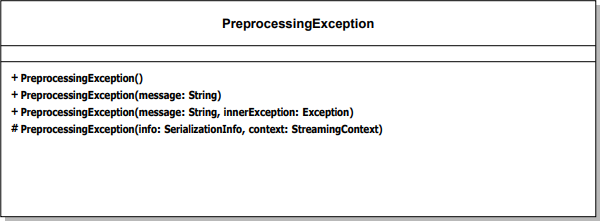
\includegraphics[width=12.5cm]{images/UML/PreprocessingException.png}}}
    \end{figure}\\

    \bk

    \paragraph*{Program \textit{(Class)}} \mbox{} \\

    \begin{figure}[H]
        \centering
        \subfloat[\centering Program Class Diagram]{{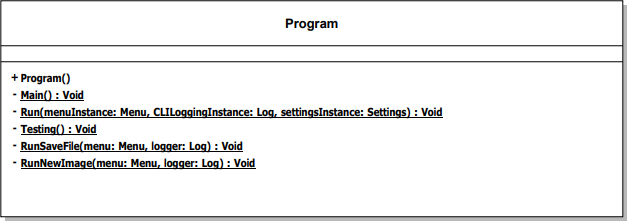
\includegraphics[width=12.5cm]{images/UML/Program.png}}}
    \end{figure}\\

    \bk

    \paragraph*{Progress Bar \textit{(Class)}} \mbox{} \\

    \begin{figure}[H]
        \centering
        \subfloat[\centering Progress Bar Class Diagram]{{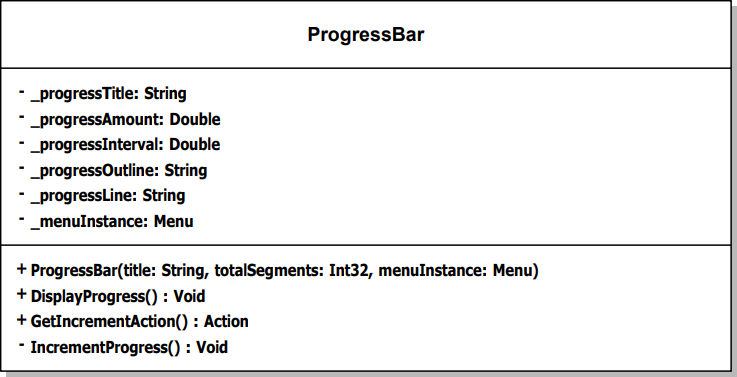
\includegraphics[width=12.5cm]{images/UML/ProgressBar.png}}}
    \end{figure}\\

    \bk

    \paragraph*{Queue \textit{(Class)}} \mbox{} \\

    \begin{figure}[H]
        \centering
        \subfloat[\centering Queue Class Diagram]{{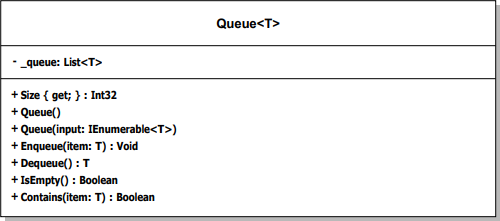
\includegraphics[width=12.5cm]{images/UML/Queue.png}}}
    \end{figure}\\

    \bk

    \paragraph*{Raw Image \textit{(Structure)}} \mbox{} \\

    \begin{figure}[H]
        \centering
        \subfloat[\centering Raw Image Class Diagram]{{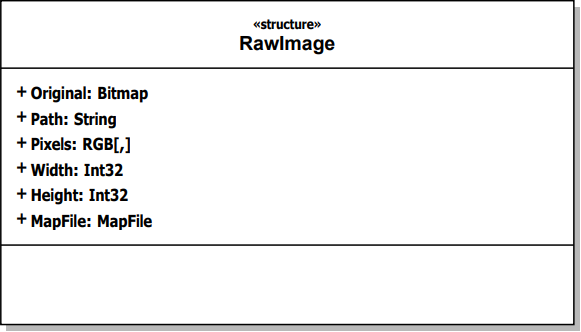
\includegraphics[width=12.5cm]{images/UML/RawImage.png}}}
    \end{figure}\\

    \bk

    \paragraph*{RGB \textit{(Structure)}} \mbox{} \\

    \begin{figure}[H]
        \centering
        \subfloat[\centering RGB Class Diagram]{{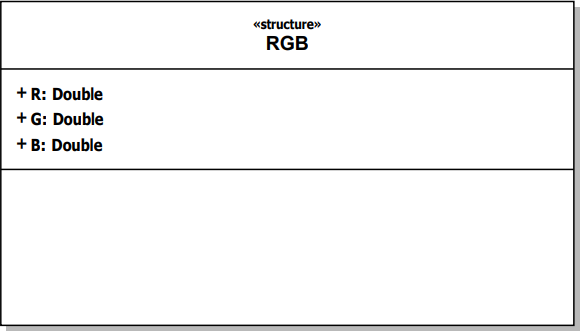
\includegraphics[width=12.5cm]{images/UML/RGB.png}}}
    \end{figure}\\

    \bk

    \paragraph*{Road Detection \textit{(Class)}} \mbox{} \\

    \begin{figure}[H]
        \centering
        \subfloat[\centering Road Detection Class Diagram]{{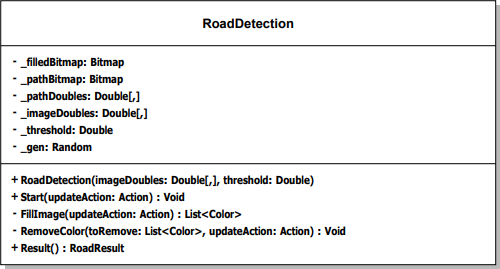
\includegraphics[width=12.5cm]{images/UML/RoadDetection.png}}}
    \end{figure}\\

    \bk

    \paragraph*{Road Result \textit{(Structure)}} \mbox{} \\

    \begin{figure}[H]
        \centering
        \subfloat[\centering Road Result Class Diagram]{{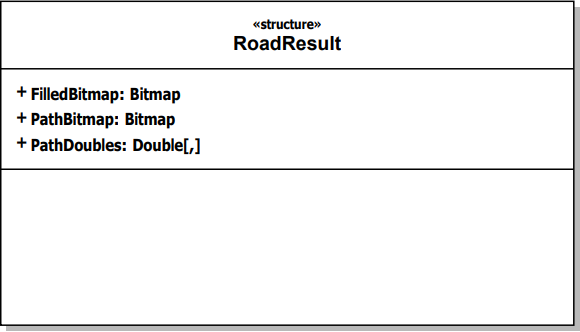
\includegraphics[width=12.5cm]{images/UML/RoadResult.png}}}
    \end{figure}\\

    \bk

    \paragraph*{Road Sequence \textit{(Class)}} \mbox{} \\

    \begin{figure}[H]
        \centering
        \subfloat[\centering Road Sequence Class Diagram]{{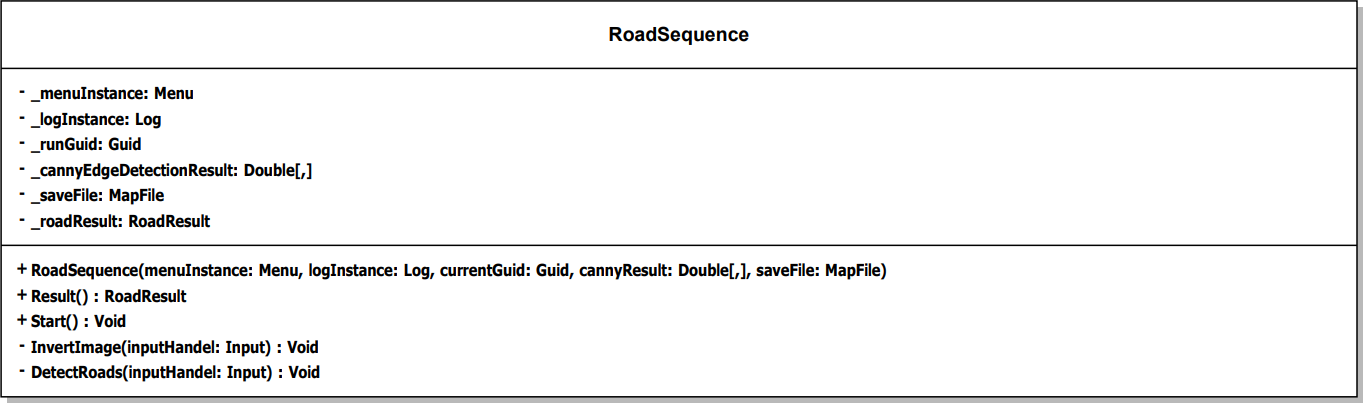
\includegraphics[width=12.5cm]{images/UML/RoadSequence.png}}}
    \end{figure}\\

    \bk

    
    \paragraph*{Save File \textit{(Class)}} \mbox{} \\

    \begin{figure}[H]
        \centering
        \subfloat[\centering Save File Class Diagram]{{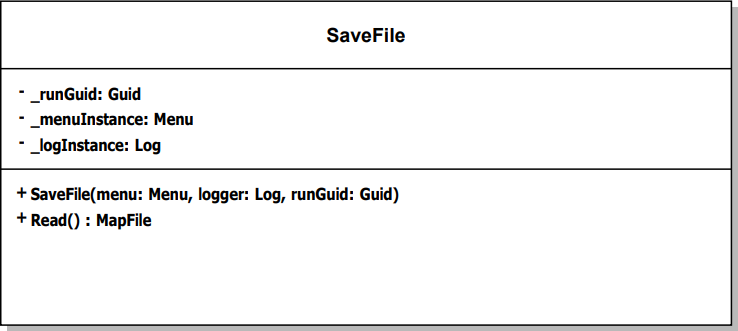
\includegraphics[width=12.5cm]{images/UML/SaveFile.png}}}
    \end{figure}\\

    \bk

    
    \paragraph*{Settings \textit{(Class)}} \mbox{} \\

    \begin{figure}[H]
        \centering
        \subfloat[\centering Settings Class Diagram]{{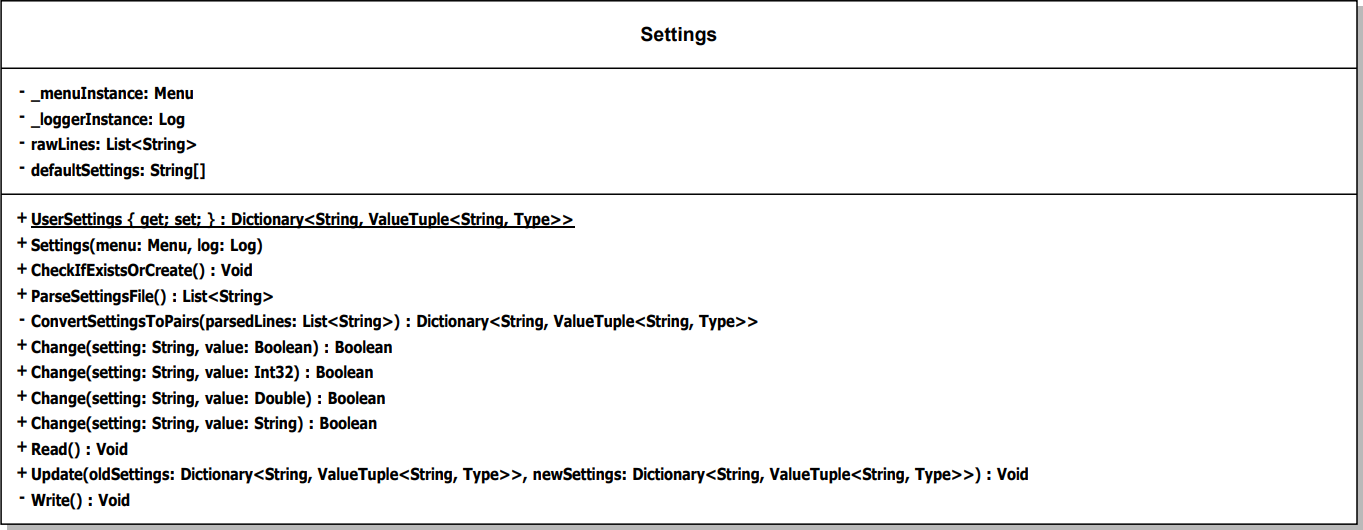
\includegraphics[width=12.5cm]{images/UML/Settings.png}}}
    \end{figure}\\

    \bk

    \paragraph*{Settings Control \textit{(Class)}} \mbox{} \\

    \begin{figure}[H]
        \centering
        \subfloat[\centering Settings Control Class Diagram]{{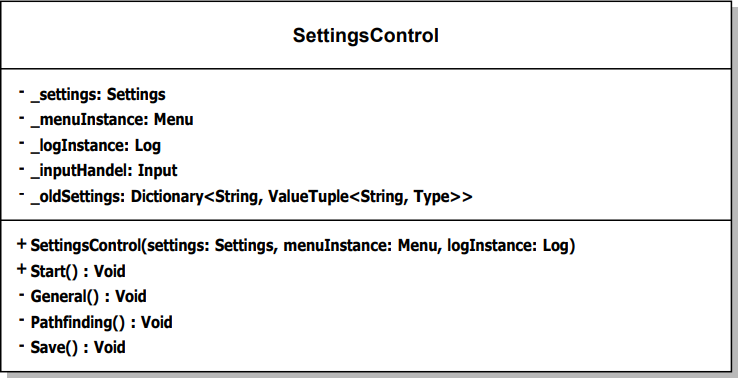
\includegraphics[width=12.5cm]{images/UML/SettingsControl.png}}}
    \end{figure}\\

    \bk

    \paragraph*{Settings Exception \textit{(Exception)}} \mbox{} \\

    \begin{figure}[H]
        \centering
        \subfloat[\centering Settings Exception Class Diagram]{{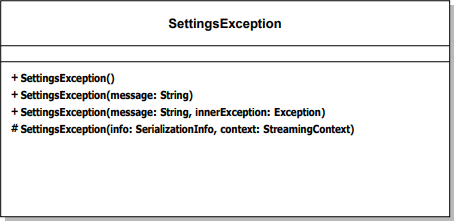
\includegraphics[width=12.5cm]{images/UML/SettingsException.png}}}
    \end{figure}\\

    \bk

    \paragraph*{Stack \textit{(Class)}} \mbox{} \\

    \begin{figure}[H]
        \centering
        \subfloat[\centering Stack Class Diagram]{{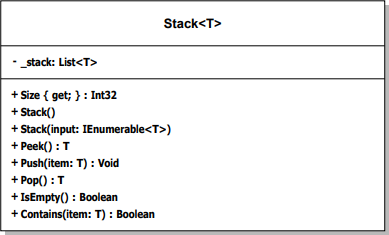
\includegraphics[width=12.5cm]{images/UML/Stack.png}}}
    \end{figure}\\

    \bk

    \paragraph*{Structures \textit{(Class)}} \mbox{} \\

    \begin{figure}[H]
        \centering
        \subfloat[\centering Structures Class Diagram]{{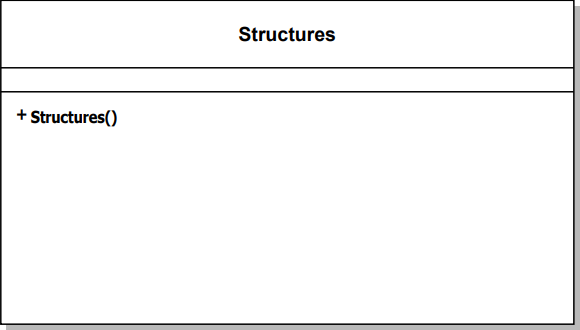
\includegraphics[width=12.5cm]{images/UML/Structures.png}}}
    \end{figure}\\

    \bk

    \paragraph*{Sync Edge Detection \textit{(Class)}} \mbox{} \\

    \begin{figure}[H]
        \centering
        \subfloat[\centering Sync Edge Detection Class Diagram]{{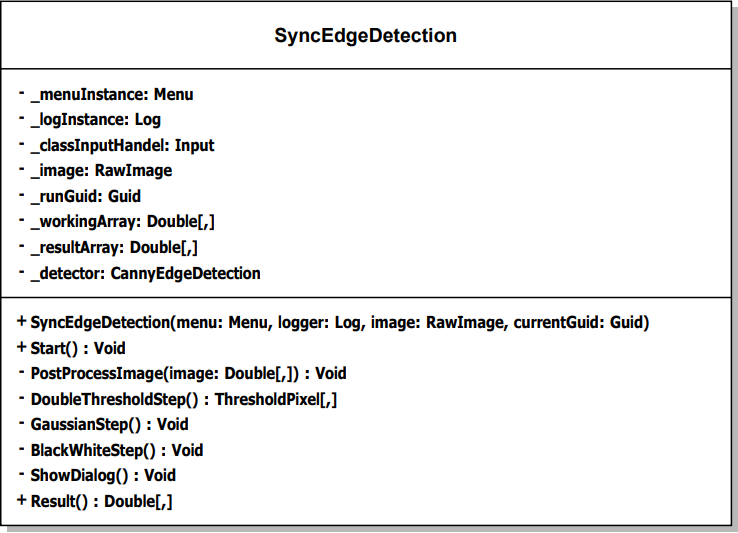
\includegraphics[width=12.5cm]{images/UML/SyncEdgeDetection.png}}}
    \end{figure}\\

    \bk


    \paragraph*{Text Wall \textit{(Class)}} \mbox{} \\

    \begin{figure}[H]
        \centering
        \subfloat[\centering Text Wall Class Diagram]{{\includegraphics[width=12.5cm]{images/UML/TextWall.png}}}
    \end{figure}\\

    \bk

    \paragraph*{Threshold Pixel \textit{(Structure)}} \mbox{} \\

    \begin{figure}[H]
        \centering
        \subfloat[\centering Threshold Pixel Class Diagram]{{\includegraphics[width=12.5cm]{images/UML/ThresholdPixel.png}}}
    \end{figure}\\

    \bk

    \paragraph*{Traversal \textit{(Class)}} \mbox{} \\

    \begin{figure}[H]
        \centering
        \subfloat[\centering Traversal Class Diagram]{{\includegraphics[width=12.5cm]{images/UML/Traversal.png}}}
    \end{figure}\\

    \bk

    \paragraph*{Utility \textit{(Class)}} \mbox{} \\

    \begin{figure}[H]
        \centering
        \subfloat[\centering Utility Class Diagram]{{\includegraphics[width=12.5cm]{images/UML/Utility.png}}}
    \end{figure}\\

    \bk

    \paragraph*{View Image Form \textit{(Windows Form)}} \mbox{} \\

    \begin{figure}[H]
        \centering
        \subfloat[\centering View Image Form UML Diagram]{{\includegraphics[width=12.5cm]{images/UML/ViewImageForm.png}}}
    \end{figure}\\

    \BK

    \subsection{File Structure}
    % TODO
    \subsubsection{Program Files}
    \bk
    \subsubsection{Generated Files}
    \bk

    \BK

    \subsection{Algorithms}

    \subsubsection{Edge Detection}
    This has been explained in detail in the class breakdown and analysis sections of this report. Here I will explain the general idea behind edge detection as a whole and what method it plays here. \\ \bk

    The purpose of edge detection is to allow an application to pick out the edges of a common example of this is in parcel courier services where when a parcel is being shipped they will need to be able to find the exact dimensions of the parcel but cannot afford to have someone there to measure every one. In this case edge detection can be used in order to find the outline and therefore allow it to be processed. The relevance of this to my program is that I need to be able to pick out, on a given image, where the roads are. This I feel is a perfect application of edge detection since I will be picking out roads which are characterised by edges on an image. \\ \bk

    There are several different methods of edge detection, the ones which I came across during my research are all examples of searching. Examples of the methods I came across are, Canny (the method I chose), Kovalevsky which takes a rather different approach to Canny where this one uses the second differential of regions in the image to work iut where there are changes in intensity and finally Sobel detection. This is somewhat incorporated into Canny edge detection however the theory behind this is purley mathematical. It involve taking remade matrices and multiplying the image with them. \\ \bk

    The advantage to Canny edge detection is that it has two major advantages:
    \begin{itemize}
        \item High Quality Maps: The way in which the image is processed allows it to preserve the resolution as it flows through the various steps. I want to be able to keep the image as high quality as possible since this is presented to a user and not being used in a machine learning environment.
        \item Accuracy: This method in particular with the first step of the Gaussian filtering, allows the inputs to be noisy, such as a photographed image. This means that I don't have to worry about de-noising the image first. 
    \end{itemize}

    \bk

    \subsubsection{Refinement Algorithm (Custom)}
    This is part of the processing the map into a a computer recognisable form. The stage after this will be filling the image. In order to do this the program must have a closed shape in which it can fill. In order to do this I needed to take the output of the edge detection and make sure that all of the roads where enclosed. \\ \bk

    I have been unable to find a suitable existing algorithm to complete this for me. There are several different types of filling algorithm which will be explained soon. What I did come across in my research is that there are many different types of image kernel and how they can be used to alter image properties. One useful one which I came across was was the embossing kernel. This goes over the images and essentially "bolds" all of the lines in the image. \\ \bk

    With these "bolded lines" it can cause gaps which previously existed to be filled. However there is one final issue which is where the lines have been connected there are intermittent black pixels which haven't been fixed by the embossing kernel. In order to remedy this I will employ a similar method as the hysteresis algorithm in canny edge detection. \\ \bk
    
    The solution I have come up with is to run over every pixel in the edge map. If there are more than a set number of white "strong" pixels around a black pixel then the black will be replaced with white. What this accomplishes is a "filling" the black pot holes. Overall this does not accomplish much however it means that if an image needs more than one pass of this "fortification" algorithm then this makes the result more reliable in the long run. \\ \bk

    I have also decided that this will need to have the option of being run more than once. I found that during the testing if there where large gaps then the embossing would need to occurs more than once.\\
    \bk

    \subsubsection{Flood Fill}
    This is an algorithm as old as time, I decided to go with th 8 direction flood fill. The premise behind the flood filling algorithm is to start from a seed point in the image and then spread the fill color to all connected pixels in the same region. The algorithm uses a queue to store the pixels that need to be filled, and it works by visiting each pixel in the queue, checking its 8 neighbouring pixels, and adding any unvisited pixels that belong to the same region to the queue. This process continues until all pixels in the region have been visited and filled. \\ \bk

    The algorithm can be implemented in a variety of ways, and it is often used as a building block for more complex image processing, as is being used in this case, algorithms, such as object recognition, image segmentation, and feature extraction. It is also commonly used in video games and user interface design to fill shapes and create smooth animations. \\ \bk

    In my version the other advantage to using the flood fill colours is that it can be shown to the user to clearly outline where the regions where which would allow them to change the thresholds and behaviour of the filling algorithm. Certain things that can be changed are the method of storing the pixels. Either in a queue of a stack. \\ 
    \bk

    \subsubsection{Area Rectification (Custom)}
    \bk

    \subsubsection{Graph Conversion (Custom)}
    \bk

    \subsubsection{Dijkstra's Search Algorithm}
    Dijkstra's search algorithm is a graph search algorithm that is commonly used to find the shortest path between two nodes in a graph. It was first proposed by the Dutch computer scientist Edsger W. Dijkstra in 1956, and it is widely used in computer science, especially in the fields of computer networking, transportation systems, and geographic information systems (similar to my program here). \\ \bk

    The algorithm works by maintaining a priority queue of nodes that have been visited and continually updating the distance to the nearest unvisited node until the destination node has been reached. The algorithm operates as follows:\\

    \begin{itemize}
    \item Start at the source node and set the distance to the source node to zero.

    \item Visit the neighbors of the current node and update their distances based on the distance to the current node and the edge weight between the current node and the neighbors.

    \item Choose the node with the smallest distance as the next node to visit, and mark it as visited. Repeat the process until the destination node has been reached or all nodes have been visited.
    \end{itemize}

    Dijkstra's algorithm is guaranteed to find the shortest path between two nodes in a graph if there are no negative edge weights. The algorithm is efficient and can be implemented in a variety of programming languages, including C#.\\ \bk

    In this map processing project, Dijkstra's algorithm can be used to find the shortest path between two points on a map, which can be useful for navigation, route planning, and other applications. The algorithm can be adapted to work with different types of maps, such as road networks or public transportation systems, by representing the map as a graph and defining the edge weights between nodes based on the specific requirements of this application. \\ \bk

    As I mentioned really usefully for this application because if I could expand the application to work out the weights of different roads based on width. \\ 
    \bk
    
    \subsubsection{A-Star Search Algorithm}
    A* is a graph search algorithm that is commonly used to find the shortest path between two nodes in a graph. It was first proposed by Peter Hart, Nils Nilsson, and Bertram Raphael in 1968 and is considered an extension of Dijkstra's algorithm. \\ \bk

    Like Dijkstra's algorithm, A* operates by maintaining a priority queue of nodes that have been visited, and it continually updates the distance to the nearest unvisited node until the destination node has been reached. The key difference between A* and Dijkstra's is that A* incorporates a heuristic function to estimate the remaining distance from a node to the destination node. This heuristic function allows A* to prioritize nodes that are likely to be closer to the destination node, making it more efficient than Dijkstra's algorithm in many cases. \\ \bk

    The algorithm operates as follows:
    \begin{itemize}
        \item Start at the source node and set the distance to the source node to zero.
        \item Visit the neighbors of the current node and update their distances based on the distance to the current node, the edge weight between the current node and the neighbors, and the estimated remaining distance to the destination node.
        \item Choose the node with the smallest estimated total distance (the sum of the distance to the current node and the estimated remaining distance to the destination node) as the next node to visit, and mark it as visited. Repeat the process until the destination node has been reached or all nodes have been visited.
    \end{itemize}

    A* is often used in computer science and engineering applications that require finding the shortest path between two nodes in a graph, such as computer graphics, video game development, robotics, and artificial intelligence. In this map processing project, A* can be used to find the shortest path between two points on a map, taking into account factors such as road conditions, traffic, and elevation, to provide an optimal route for navigation and route planning which adapts to given conditions. \\ \bk

    Then overriding main reason which I am choosing to go with a validation of A* with cartesian distance is that it is significantly faster and more efficient than Dijkstra's. Although Dijkstra has the advantage of post routing meaning that as long as the start node is the same the route can be found instantly. 
    \bk

    \subsubsection{Binary Heap Min Priority Queue}
    A binary heap is a type of data structure that can be used to implement a priority queue, where elements are kept in order based on their priority. A binary heap can be either a min-heap or a max-heap, depending on whether the smallest or largest element is considered to have the highest priority. In a min-heap, the parent node of the heap has a value that is less than or equal to the values of its children.\\ \bk

    A binary heap is implemented as a complete binary tree, where all levels of the tree are filled except possibly the last one, which is filled from left to right. In a min-heap, the smallest element is stored at the root of the tree, and the two children of a node with a smaller value are stored in the left and right child nodes of that node.\\ \bk
    
    To implement a min-priority queue using a binary heap, we can use the following operations;\\ \bk

    Insertion: To insert an element into the binary heap, it is added to the next available position in the last level of the tree, and then "bubbled up" the tree by swapping it with its parent until the min-heap property is restored.\\ \bk
    
    Extraction of minimum element: To extract the minimum element from the binary heap, we remove the root node and replace it with the last element in the tree. The new root node is then "sunk down" the tree by swapping it with its smaller child until the min-heap property is restored.\\ \bk
    
    Decrease key: To decrease the priority of an element in the binary heap, we first find the element and update its value, and then "bubble up" the node by swapping it with its parent until the min-heap property is restored.\\ \bk
    
    Binary heaps are used in many algorithms, such as Dijkstra's shortest path algorithm and the A* algorithm which happen to be the exact algorithms I am using, because they have the property of being able to efficiently maintain a priority queue in a sorted order. They have a time complexity of O(log n) for inserting and extracting elements, which makes them a fast and efficient data structure for implementing priority queues, keeping the delay of processing low.\\ \bk

    \bk








\end{FlushLeft}